\chapter{\Dijet Azimuthal Decorrelations}
\label{chap:azimuthal-decorrelation}

\chapterquote{I believe there is a direct correlation between love and laughter.}
{Yakov Smirnoff}

\section{Introduction}
At leading order, \dijet production results in two jets being produced which are
completely anti-correlated in azimuthal angle: satisfying $\DeltaPhi = \pi$. With
the addition of soft radiation or higher order jet production, the opening angle
between the jets will deviate from this idealised case (see \FigureRef{fig:azimuthal-decorrelation:dPhi_diagram}).
Thus azimuthal decorrelation tests both higher order perturbative \QCD and the
modelling of non-perturbative soft processes.

\begin{figure}[htpb]
  \subfloat[$\DeltaPhi \simeq \pi$ for \dijet{s}]{
    \includegraphics[width=\tinyfigwidth]{chapters/azimuthal-decorrelation/dPhi.backtoback.eps}
    \label{fig:azimuthal-decorrelation:back_to_back}}
  \quad
  \subfloat[$\DeltaPhi < \pi$ with soft radiation]{
    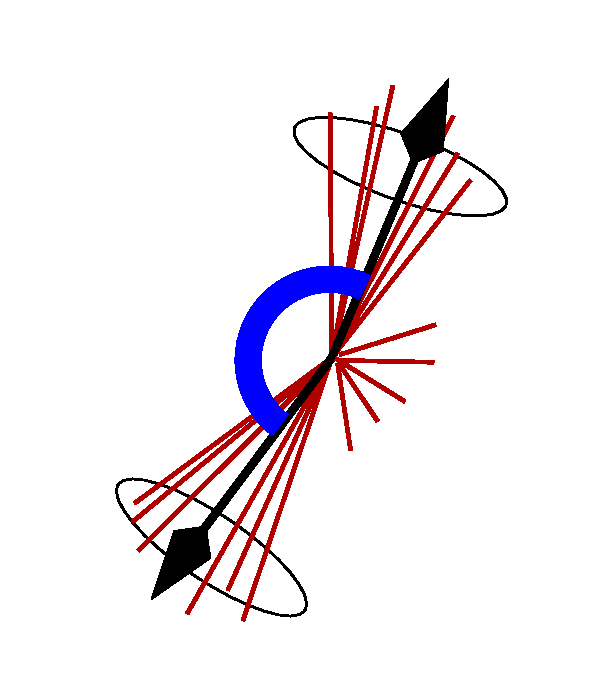
\includegraphics[width=\tinyfigwidth]{chapters/azimuthal-decorrelation/dPhi.soft.eps}
    \label{fig:azimuthal-decorrelation:soft_radiation}}
  \quad
  \subfloat[$\DeltaPhi < \pi$ with third jet]{
    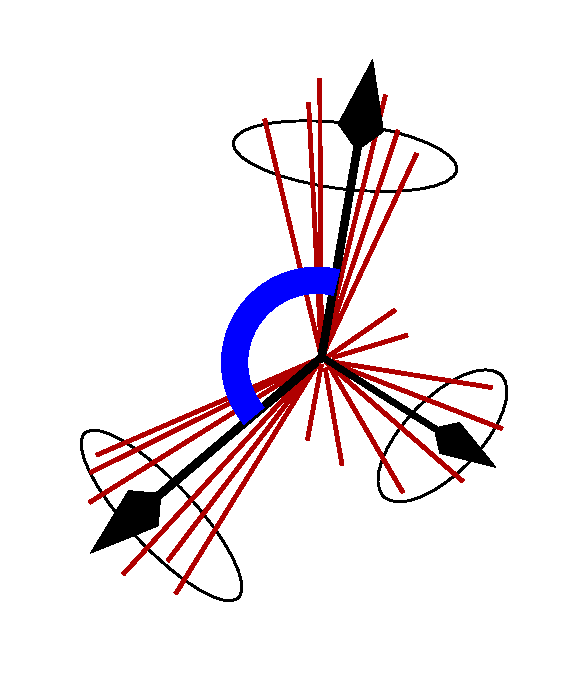
\includegraphics[width=\tinyfigwidth]{chapters/azimuthal-decorrelation/dPhi.thirdjet.eps}
    \label{fig:azimuthal-decorrelation:third_jet}}
  \caption{\Dijet configurations and resulting \DeltaPhi in jet events. As the amount
           of \QCD radiation in the event increases (from left to right), the azimuthal
           angle (shown in blue) between the two leading jets in the event decreases.}
  \label{fig:azimuthal-decorrelation:dPhi_diagram}
\end{figure}

Studying azimuthal decorrelations probes similar physics to the \dijet with a
jet veto study discussed in \ChapterRef{chap:gbj}. It therefore makes sense to
attempt to integrate these two measurements by constructing observables which
combine angular information with jet vetoes.

\section{Event Selection}
As was the case for the previously discussed jet veto measurement, events are required to belong to a good
run and to have exactly one good primary vertex, as discussed in \SectionRef{sec:gbj:event_selection}.
Jets are then reconstructed using one of the \ATLAS standard jet parameter sets:
\akt jets with $R =0.6$ (see \SectionRef{bg-theory:recombination_algorithms} and
\SectionRef{sec:analysis-tools:jet_reconstruction}). Events are rejected if they
contain any jets with $\pT > \unit{20}{\GeV}$ that are flagged as ``bad'' or
``ugly'' by the standard loose jet cleaning cuts.

After these cuts have been applied, the boundary jets are taken as the two highest
\pT jets with $|\rap| < 4.4$. Provided that the leading jet satisfies $\pT > \unit{60}{\GeV}$
and the second jet $\pT > \unit{50}{\GeV}$, the event is accepted as an inclusive
event. Gap events are defined as the subset of inclusive events that do not contain
an additional jet with \pT greater than the veto scale, $\Qnought = \unit{20}{\GeV}$.

\section{Observables}
This analysis measures quantities in terms of the gap fraction, that fraction of
accepted events which do not possess a third jet with $\pT > \Qnought$. The gap
fraction is measured as a function of both \DeltaY and the jet veto scale,
\Qnought. 

The decorrelation between \DeltaPhi and \DeltaY is primarily studied through the variables
\meanCosDPhi and \meanCosTwoDPhi. Theoretical predictions~\cite{Colferai:2011:NLLBFKL}
indicate that these quantities could provide discriminating power to distinguish
between DGLAP and \BFKL-like evolutions: distributions of \meanCosDPhi and \meanCosTwoDPhi
are therefore constructed as functions of \DeltaY.

Finally, double differential \xs{s} as a function of \DeltaY and \DeltaPhi, \cosDPhi
or \cosTwoDPhi are calculated separately for gap and inclusive events, using a jet veto at
$\Qnought = \unit{20}{\GeV}$.

\section{Trigger Strategy}
As this measurement extends out to $\DeltaY = 8$, the strategy used in \SectionRef{sec:gbj:triggers}
cannot be used, since the assumption that all events will have at least one central
jet is no longer valid. The trigger strategy used to measure the \dijet \xs is,
however, applicable since this uses both the central and forward trigger systems depending
on the \pT and rapidity of the two leading jets (see \SectionRef{sec:dijets:trigger}).

Although parameters like the optimum values for the matching cuts do not have to
be rederived, a closure test is performed with \MC to demonstrate that the gap
fraction is not biased when adopting this trigger strategy. The effects of the trigger
are emulated using the prescale values of a typical run. \MC events are discarded
at random according to these prescales and the surviving events constitute a ``triggered
pseudodata'' sample, which is then analysed with the same procedure as is used
for data. 

The resulting gap fraction spectrum is shown in \FigureRef{fig:azimuthal-decorrelation:closure_dY}
as a function of the rapidity difference, \DeltaY, and in \FigureRef{fig:azimuthal-decorrelation:closure_Q0}
as a function of the veto scale, \Qnought. The pseudodata distributions obtained after
trigger emulation and correction for prescale are compatible within $\sim1\%$
with the same distributions from the original \MC sample without the trigger
requirement, validating the two trigger method for this measurement.

\begin{figure}[htpb]
  \subfloat[Closure as a function of \DeltaY]{
    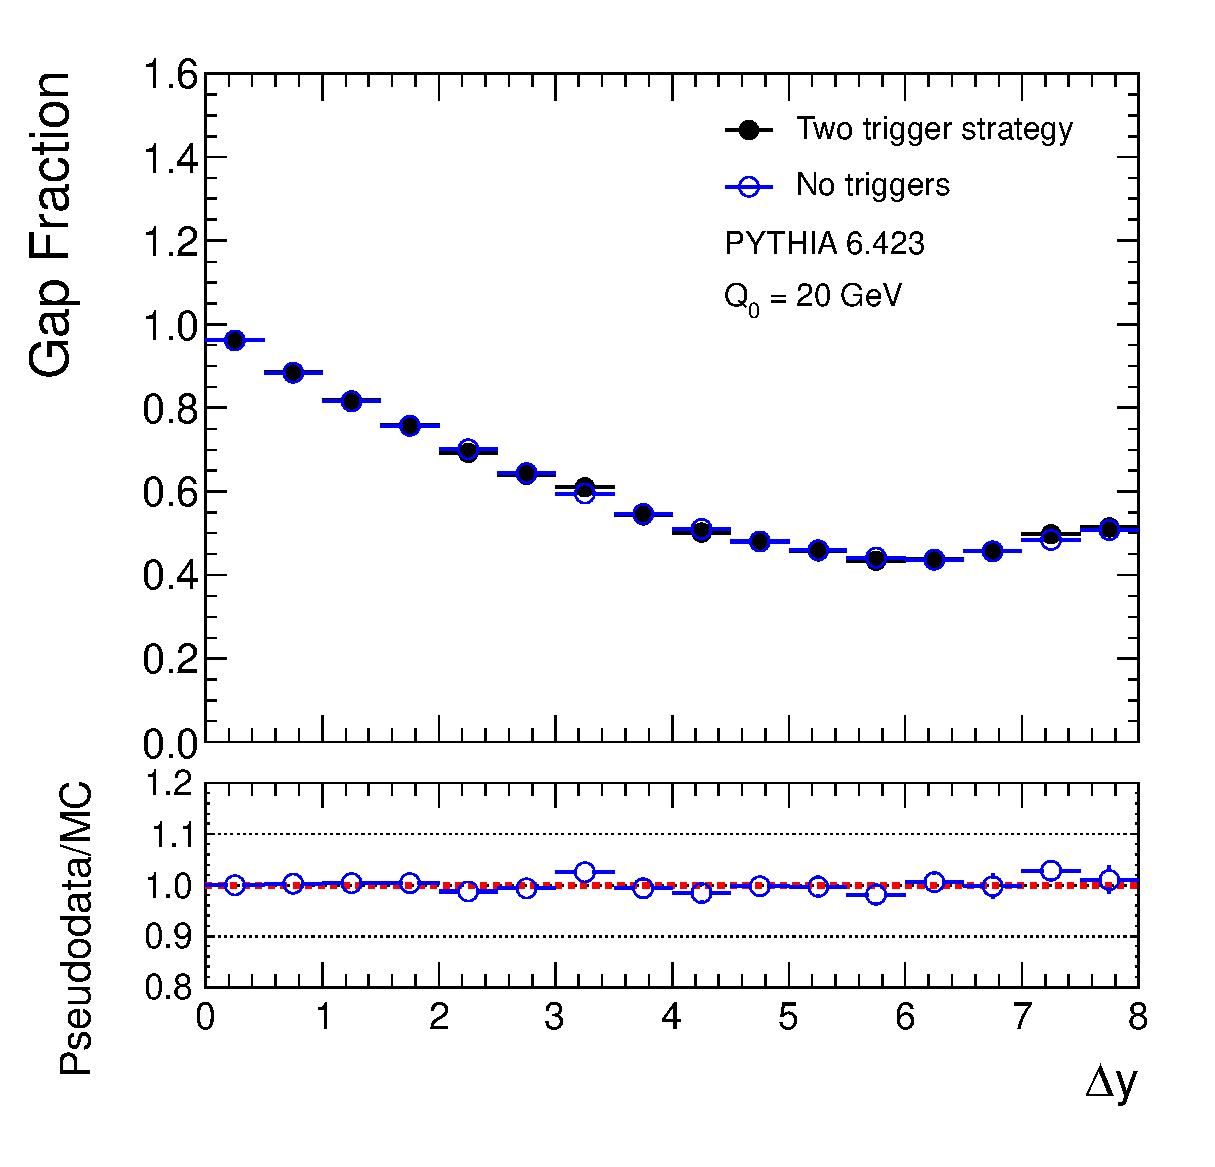
\includegraphics[width=\smallfigwidth]{chapters/azimuthal-decorrelation/Closure.GapFraction.Q0_20.dYBins.eps}
    \label{fig:azimuthal-decorrelation:closure_dY}}
  \quad
  \subfloat[Closure as a function of \Qnought]{
    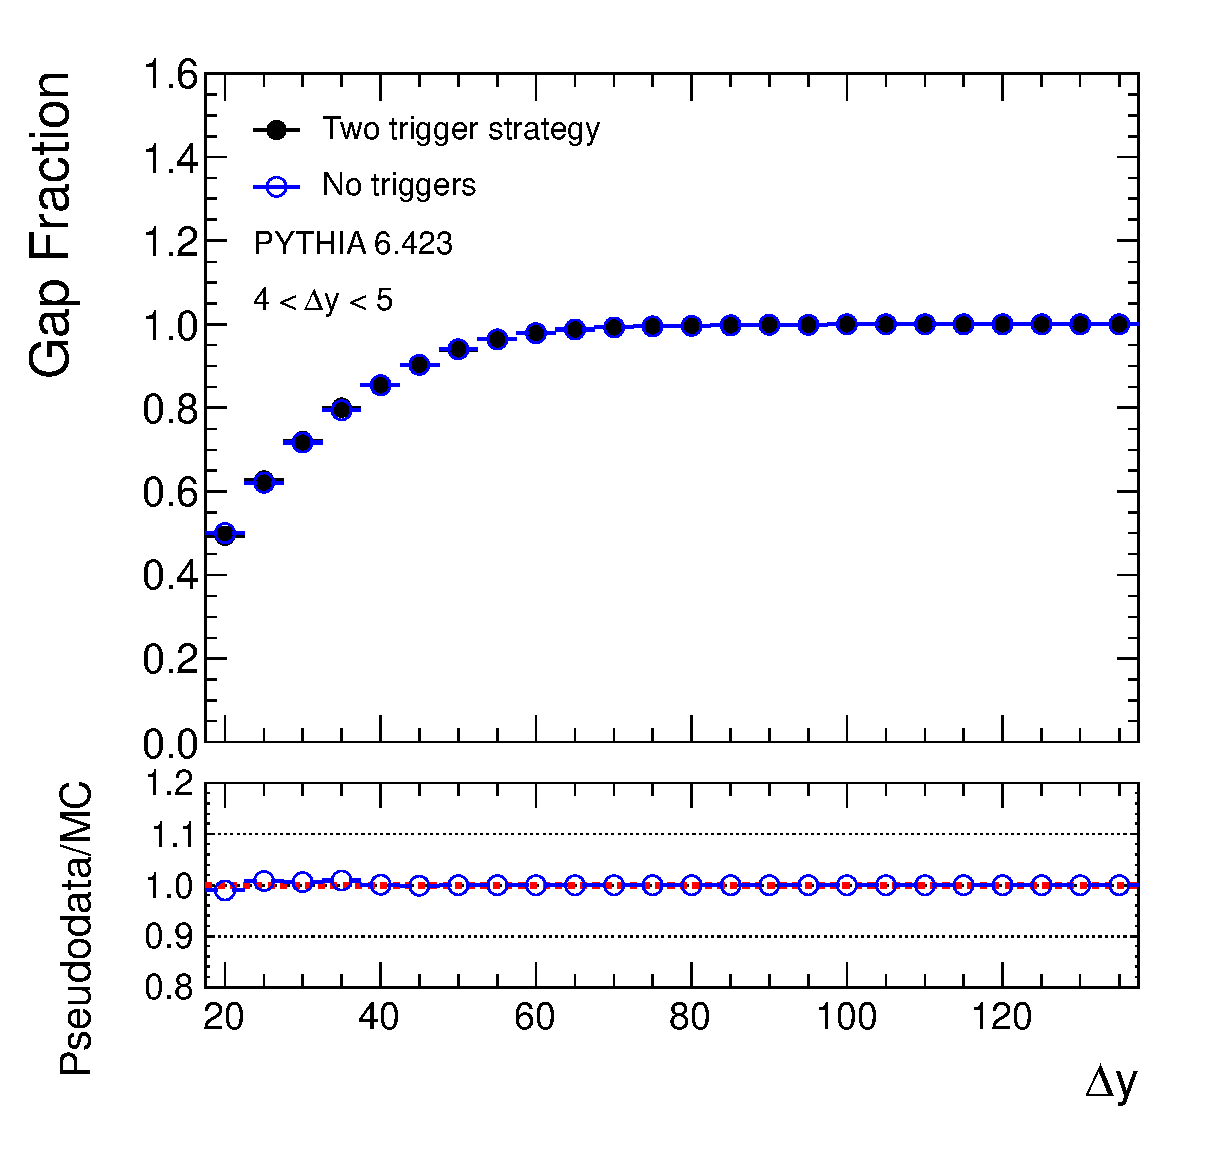
\includegraphics[width=\smallfigwidth]{chapters/azimuthal-decorrelation/Closure.GapFraction.4dY5.Q0Bins.eps}
    \label{fig:azimuthal-decorrelation:closure_Q0}}
  \caption{Summary plot of the closure test for a \dijet \MC sample for jets identified
           using the \akt algorithm with $R=0.6$. The black dots represent the result
           of emulating the trigger in the \MC and then correcting for it
           using the same technique used on data, while the blue dotted lines represent
           the result of analysing all events, without trigger corrections. This
           test is conducted \protect\subref{fig:azimuthal-decorrelation:closure_dY} as
           a function of \DeltaY and \protect\subref{fig:azimuthal-decorrelation:closure_Q0}
           as a function of\Qnought.}
  \label{fig:azimuthal-decorrelation:closure}
\end{figure}

\section{Single Vertex Cut Efficiency}
In order to measure \xs{s}, the impact of the single vertex cut needs to be
accounted for. In early periods, with lower beam intensities, the average number
of collisions per bunch crossing was low and hence the cut efficiency was high.
In later periods, increasing pile-up means that the efficiency drops to about
20\%. To obtain accurate \xs measurements, a period-by-period correction to the
observed luminosity needs to be applied, to remove the effects of this
inefficiency. \TableRef{tab:azimuthal-decorrelation:SVefficiencies} shows the
efficiency of this cut as a function of period; the observed luminosities are
reduced by the same fraction before the final \xs results are produced.

\begin{table}
\begin{center}
  \begin{tabular}{ l c c c c c c c c c }
    Period     & A     & B     & C     & D     & E     & F     & G     & H     & I     \\
%    Efficiency & 0.715 & 0.924 & 0.925 & 0.571 & 0.439 & 0.354 & 0.290 & 0.276 & 0.207 \\
    Efficiency & 1.000 & 0.929 & 0.932 & 0.573 & 0.439 & 0.368 & 0.302 & 0.296 & 0.213 \\
   \end{tabular}
  \caption{Efficiency of the single vertex cut as a function of data taking
           period. The effects of this inefficiency are corrected for by
           reducing the effective luminosities in each period by the same
           fraction.}
  \label{tab:azimuthal-decorrelation:SVefficiencies}
\end{center}
\end{table}

\section{Unfolding Detector Effects}
The measured distributions are corrected for detector effects using the Bayesian
unfolding scheme as detailed in \SectionRef{sec:analysis-tools:unfolding}. Measuring
the efficiency, the extent to which particle level events remain in the same bin
at detector level, and the purity, the level of contamination in detector level bins,
for each bin is essential in order to determine the optimum binning for each distribution:
the bin sizes must be chosen such that the efficiency and the purity of each bin
remains high.

Here, when binned in one variable, either \DeltaY or \DeltaPhi, bin sizes were
altered until both efficiency and purity were above 0.8 in all bins. When binned
in both \DeltaY and \DeltaPhi simultaneously, this requirement was relaxed; both
efficiency and purity were required to be above 0.6 in all bins.

Sample efficiency distributions as a function of \DeltaY and \DeltaPhi can be
seen in \FigureRef{fig:azimuthal-decorrelation:efficiencies}, with purity
distributions as a function of \DeltaY and \DeltaPhi in \FigureRef{fig:azimuthal-decorrelation:purities}.
The trend with respect to \DeltaY that can be seen in the efficiency and purity for gap events, an initial decrease
followed by a flattening out, is explained by the kinematics of the observable.
Due to the steeply falling \pTthree distribution, it is likely that events which
satisfy the gap criteria at particle level, will contain a third jet with \pTthree
just below the veto scale; small differences in \pT between particle level and detector
level can mean that such events will fail the gap event selection cuts at detector
level. As \DeltaY increases, the chances of this happening increase too, before
flattening out due to the reduced phase-space which is available after requiring 
two hard high \rap jets - this effect can also be seen in \FigureRef{fig:azimuthal-decorrelation:nGapJets},
which shows the distribution of number of jets in the gap.

\begin{figure}[htpb]
  \subfloat[\DeltaY efficiency]{
    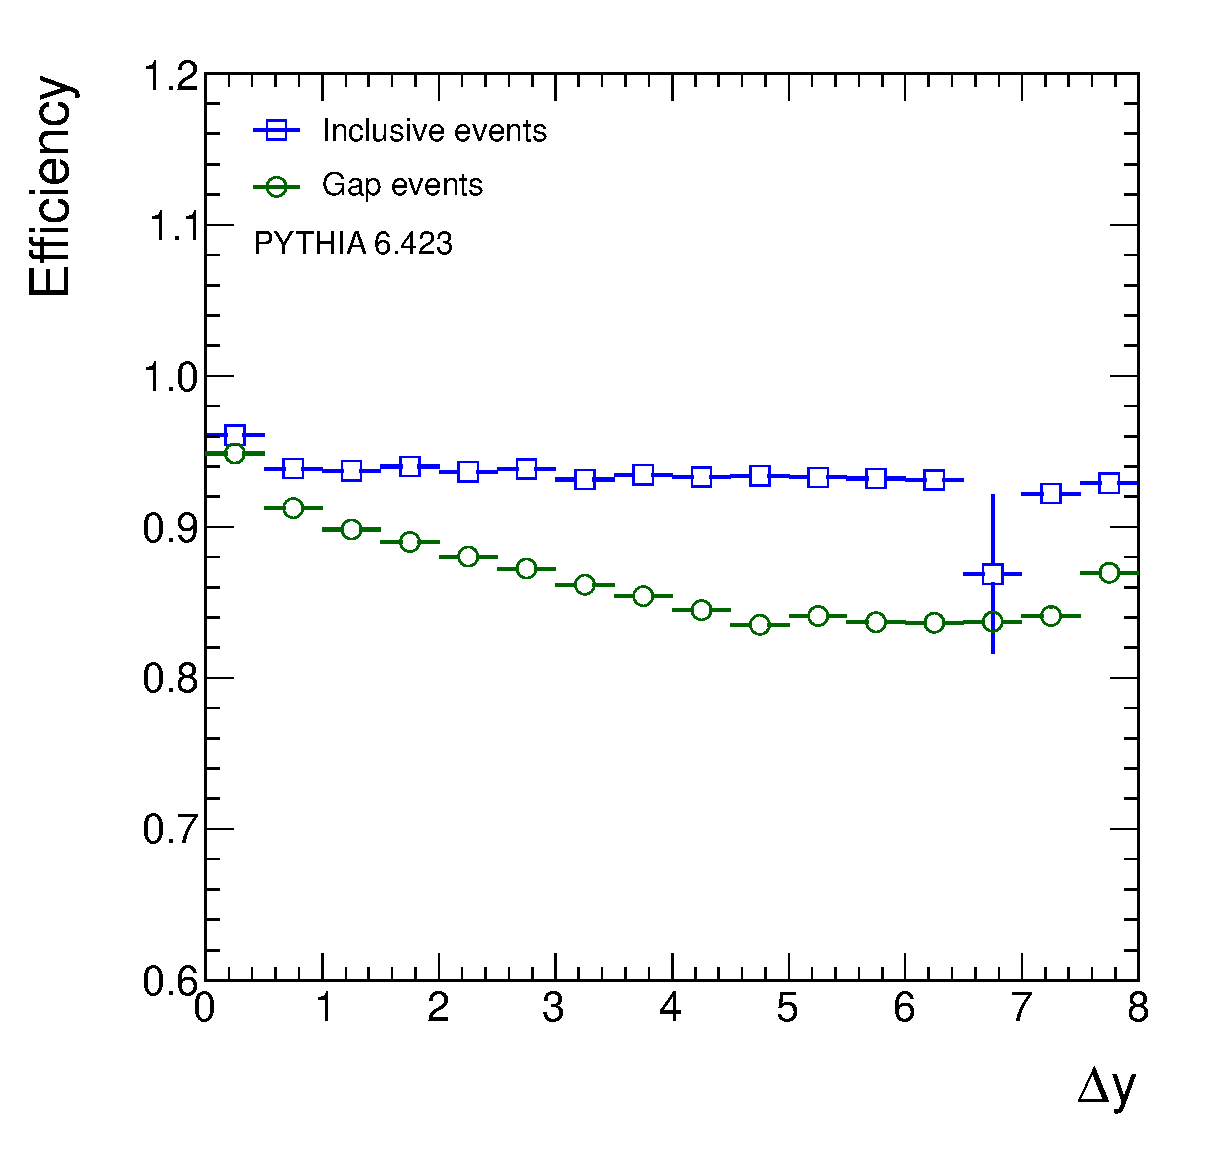
\includegraphics[width=\smallfigwidth]{chapters/azimuthal-decorrelation/Efficiency.dYBins.eps}
    \label{fig:azimuthal-decorrelation:efficiency_dY}}
  \quad
  \subfloat[\DeltaPhi efficiency for $4 \leq \DeltaY < 5$]{
    \includegraphics[width=\smallfigwidth]{chapters/azimuthal-decorrelation/Efficiency.DPhiBins.4dY5.eps}
    \label{fig:azimuthal-decorrelation:efficiency_dPhi}}
  \caption{Efficiency distributions showing the proportion of events at particle level
           which remain in each bin at detector level. \protect\subref{fig:azimuthal-decorrelation:efficiency_dY}
           shows the efficiency as a function of \DeltaY, while \protect\subref{fig:azimuthal-decorrelation:efficiency_dPhi}
           shows the efficiency as a function of \DeltaPhi in the region $4 \leq \DeltaY < 5$.
           Efficiencies are shown separately for inclusive events (blue) and gap events (green). Efficiencies are
           calculated using \Pythia \MC for jets identified using the \akt algorithm
           with $R=0.6$.}
  \label{fig:azimuthal-decorrelation:efficiencies}
\end{figure}

\begin{figure}[htpb]
  \subfloat[\DeltaY purity]{
    \includegraphics[width=\smallfigwidth]{chapters/azimuthal-decorrelation/Purity.dYBins.eps}
    \label{fig:azimuthal-decorrelation:purity_dY}}
  \quad
  \subfloat[\DeltaPhi purity for $4 \leq \DeltaY < 5$]{
    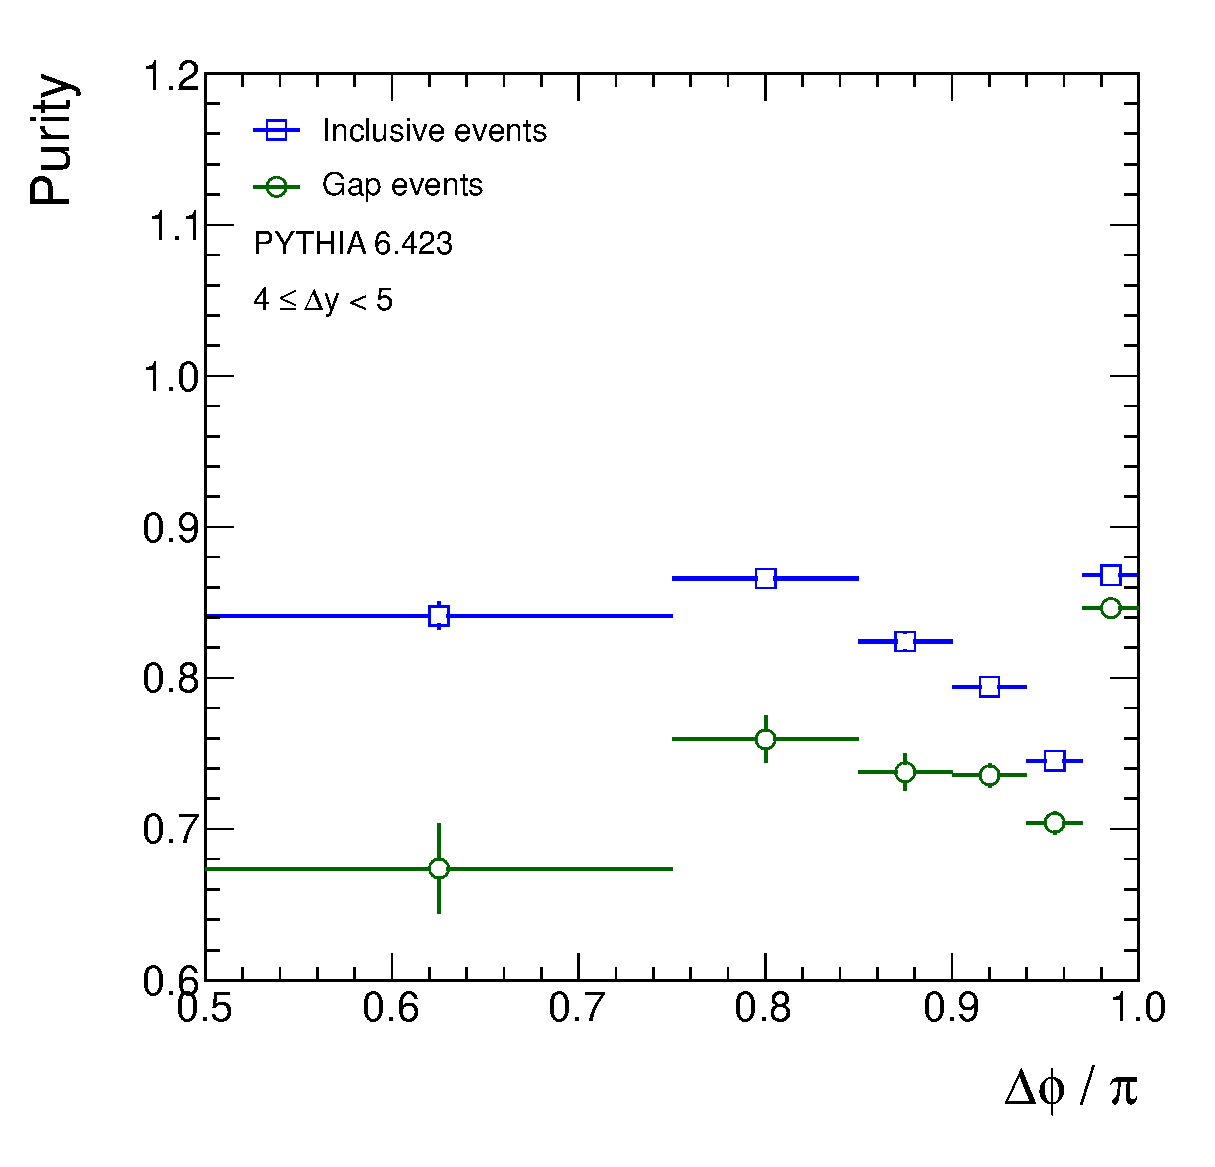
\includegraphics[width=\smallfigwidth]{chapters/azimuthal-decorrelation/Purity.DPhiBins.4dY5.eps}
    \label{fig:azimuthal-decorrelation:purity_dPhi}}
  \caption{Purity distributions showing the proportion of events in each bin at
           detector level which came from the same bin at particle level. \protect\subref{fig:azimuthal-decorrelation:purity_dY} shows
           is the purity as a function of \DeltaY, while \protect\subref{fig:azimuthal-decorrelation:purity_dPhi} shows the purity as a
           function of \DeltaPhi in the region $4 \leq \DeltaY < 5$. Purities are
           shown for inclusive events (blue) and gap events (green). Purities are
           calculated using \Pythia \MC for jets identified using the \akt algorithm
           with $R=0.6$.}
  \label{fig:azimuthal-decorrelation:purities}
\end{figure}

\FigureRef{fig:azimuthal-decorrelation:control_gap_fraction} shows the level of agreement
between \Pythia, \Herwigpp, \Alpgen and the data for two sample distributions: the
gap fraction as a function of \DeltaY and as a function of \Qnought. The only \MC
with good statistics and good agreement with data in all regions of phase space
considered here is \Pythia. Accordingly, these \Pythia samples are used to unfold
the data.

\begin{figure}[htpb]
  \subfloat[Gap fraction as a function of \DeltaY]{
    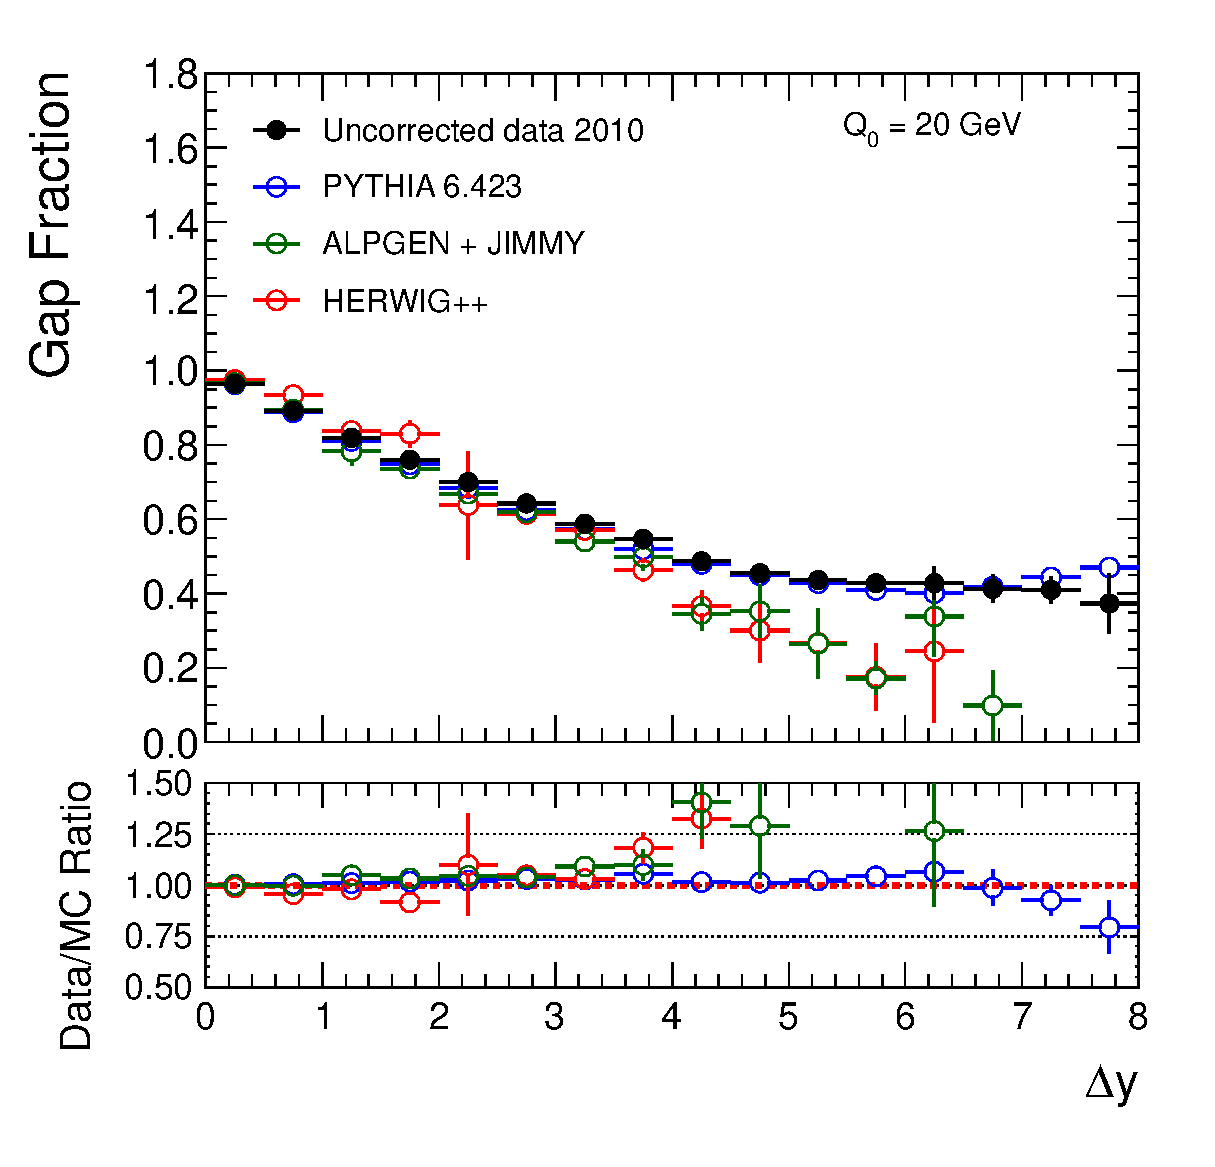
\includegraphics[width=\smallfigwidth]{chapters/azimuthal-decorrelation/Control.GapFraction.dYBins.eps}
    \label{fig:azimuthal-decorrelation:control_gap_fraction_dY}}
  \quad
  \subfloat[Gap fraction as a function of \Qnought]{
    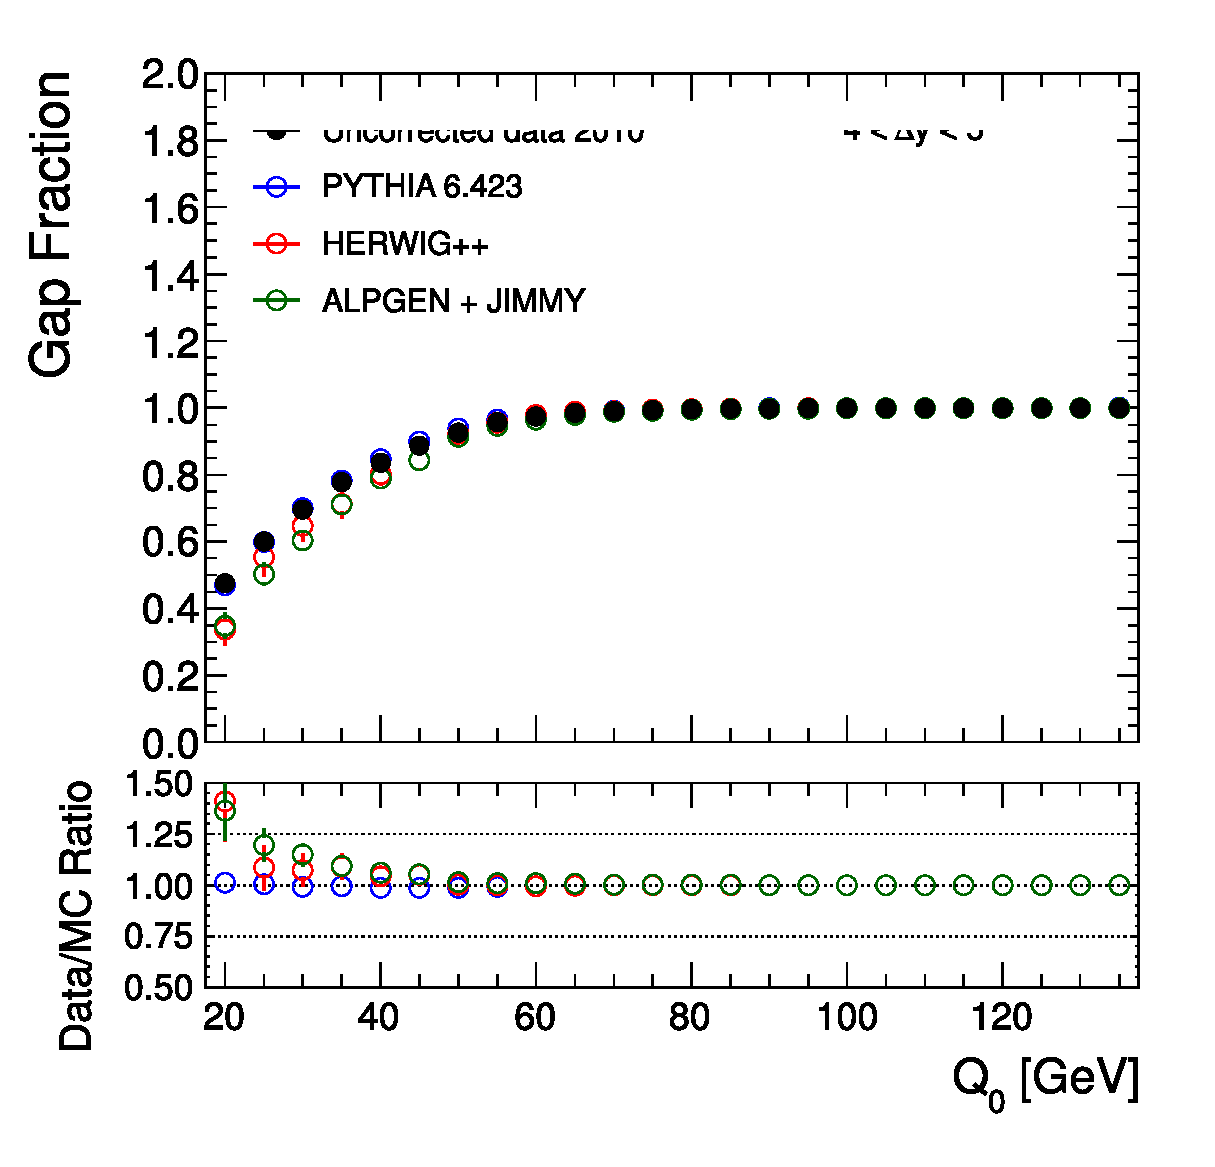
\includegraphics[width=\smallfigwidth]{chapters/azimuthal-decorrelation/Control.GapFraction.4dY5.Q0Bins.eps}
    \label{fig:azimuthal-decorrelation:control_gap_fraction_Q0}}
  \caption{Gap fraction distributions as a function of \Qnought and \DeltaY for
           jets identified using the \akt algorithm with $R=0.6$. \protect\subref{fig:azimuthal-decorrelation:control_gap_fraction_dY} shows
           the gap fraction as a function of \DeltaY for $\Qnought = \unit{20}{\GeV}$,
           while \protect\subref{fig:azimuthal-decorrelation:control_gap_fraction_Q0} shows
           the gap fraction as a function of \Qnought in the region
           $4 \leq \DeltaY < 5$. The uncorrected data are compared to the leading
           order \Pythia 6.423, \Herwigpp and \Alpgen predictions after these have
           been passed through the \ATLAS detector simulation software. The error
           bars indicate the statistical uncertainty on the measurement.}
  \label{fig:azimuthal-decorrelation:control_gap_fraction}
\end{figure}

Finally, unfolded distributions are calculated using the RooUnfold framework~\cite{Adye:2011:RooUnfold}.
This allows simultaneous comparison of multiple different unfolding methods, with
the same \MC events entering each calculation. Here simple bin-by-bin unfolding
is compared to an iterative Bayesian unfolding method~\cite{DAgostini:2010:BayesianUnfolding}
and to SVD. \FigureRef{fig:azimuthal-decorrelation:unfolding} shows sample distributions,
comparing data unfolded using each of these three methods to uncorrected, detector level data. 
Good agreement is seen between each of the unfolding methods, with the shape of the
unfolded distributions also agreeing well with the detector level data.
%Finally, unfolding factors, the multiplicative correction factors applied on a bin-by-bin
%basis to correct the data distributions for detector effects are calculated. Sample
%distributions can be seen in,
%as a function of \DeltaY and \DeltaPhi. Unfolded data are used for all results shown
%here.

\begin{figure}[htpb]
  \subfloat[Unfolded gap fraction as a function of \DeltaY]{
    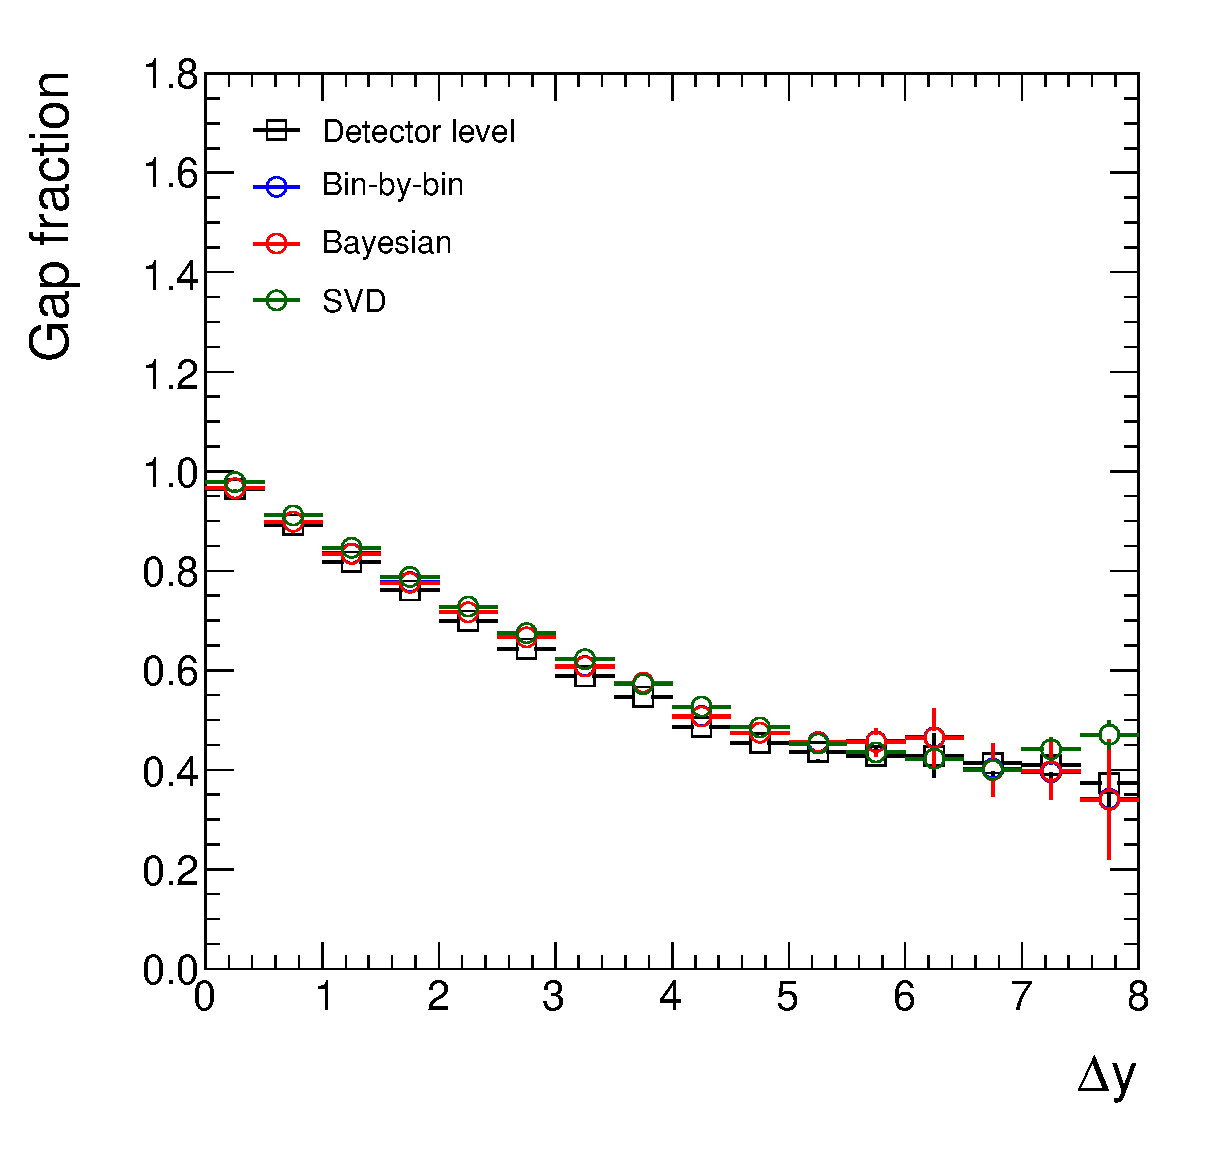
\includegraphics[width=\smallfigwidth]{chapters/azimuthal-decorrelation/Unfolded.GapFraction.dYBins.eps}
    \label{fig:azimuthal-decorrelation:unfolding_dY}}
  \quad
  \subfloat[Unfolded \xs as a function of \DeltaPhi for $2 \leq \DeltaY < 3$]{
    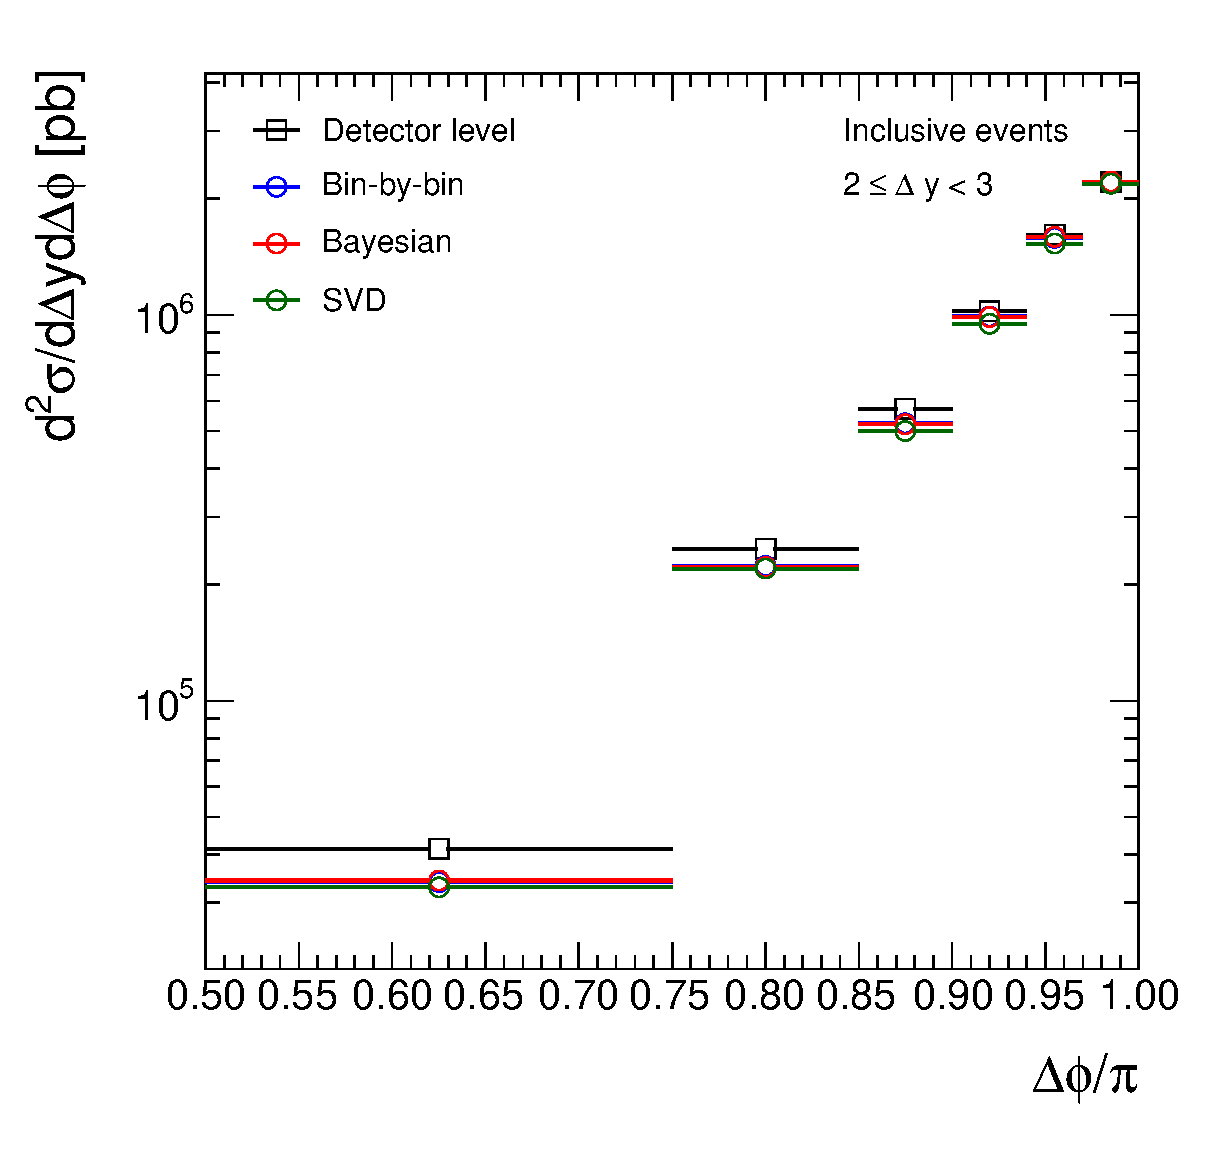
\includegraphics[width=\smallfigwidth]{chapters/azimuthal-decorrelation/Unfolded.Inclusive.CrossSection.2dY3.dPhiBins.eps}
    \label{fig:azimuthal-decorrelation:unfolding_dPhi}}
  \caption{Comparison of three different unfolding methods: bin-by-bin, Bayesian
           and SVD, showing the result of correcting measured data for detector
           effects together with the uncorrected spectrum for comparison. \protect\subref{fig:azimuthal-decorrelation:unfolding_dY}
           shows the unfolded distributions as a function of \DeltaY, while \protect\subref{fig:azimuthal-decorrelation:unfolding_dPhi}
           shows the unfolded \xs distribution as a function of \DeltaPhi
           for the region $2 \leq \DeltaY < 3$. Unfolding is performed using \Pythia
           \MC for jets identified using the \akt algorithm with $R=0.6$.}
%  \caption{Bin-by-bin unfolding factor distributions showing the value by which
%           each bin of measured data needs to be multiplied to correct for detector
%           effects. On the left are the unfolding factors as a function of \DeltaY,
%           on the right the unfolding factors as a function of \DeltaPhi in the
%           region $4 \leq \DeltaY < 5$. Unfolding factors are shown for inclusive
%           events (blue) and gap events (green). Unfolding factors are calculated
%           using \Pythia \MC for jets identified using the \akt algorithm with $R=0.6$.}
  \label{fig:azimuthal-decorrelation:unfolding}
\end{figure}

\section{Azimuthal Decorrelation Results}
\subsection{Comparison to Leading Order \MC Generators}
%For these measurements, data are only compared to leading-order \MC generators.
%Predictions from next-to-leading order generators, specifically \Powheg and \HEJ
%as in \ChapterRef{chap:gbj}, are in preparation, but the focus of this thesis is,
%anyway, on the experimental data. Unfolded data are compared against \Pythia,
%\Herwigpp and \Alpgen, all generators that are commonly used for predictive
%purposes in \ATLAS. For both data and \MC, the errors shown reflect statistical uncertainties
%only; the impact of systematic effects has not yet been determined. \FigureRef{fig:azimuthal-decorrelation:gap_fraction}
%shows the gap fraction as a  function of \DeltaY and as a function of \Qnought in the
%case that the boundary jets satisfy $4 \leq \DeltaY < 5$. Divergences between
%the \MC predictions can be seen at high \DeltaY and at low \Qnought, although
%\Pythia agrees well throughout.
For these measurements, data are initially compared to leading-order \MC generators.
predictions from next-to-leading order generators, specifically \Powheg and \HEJ
as in \ChapterRef{chap:gbj}, are also shown, but the focus of this thesis is,
anyway, on the experimental data. Unfolded data are compared against \Pythia,
\Herwigpp and \Alpgen, all generators that are commonly used for predictive
purposes in \ATLAS. For both data and \MC, the errors shown reflect statistical
uncertainties only.  %the impact of systematic effects has not yet been determined.

\FigureRef{fig:azimuthal-decorrelation:gap_fraction}
shows the gap fraction as a  function of \DeltaY and as a function of \Qnought in the
case that the boundary jets satisfy $4 \leq \DeltaY < 5$. Divergences between
the \MC predictions can be seen at high \DeltaY and at low \Qnought, although
\Pythia agrees well throughout.

\begin{figure}[htpb]
  \subfloat[Gap fraction as a function of \DeltaY]{
    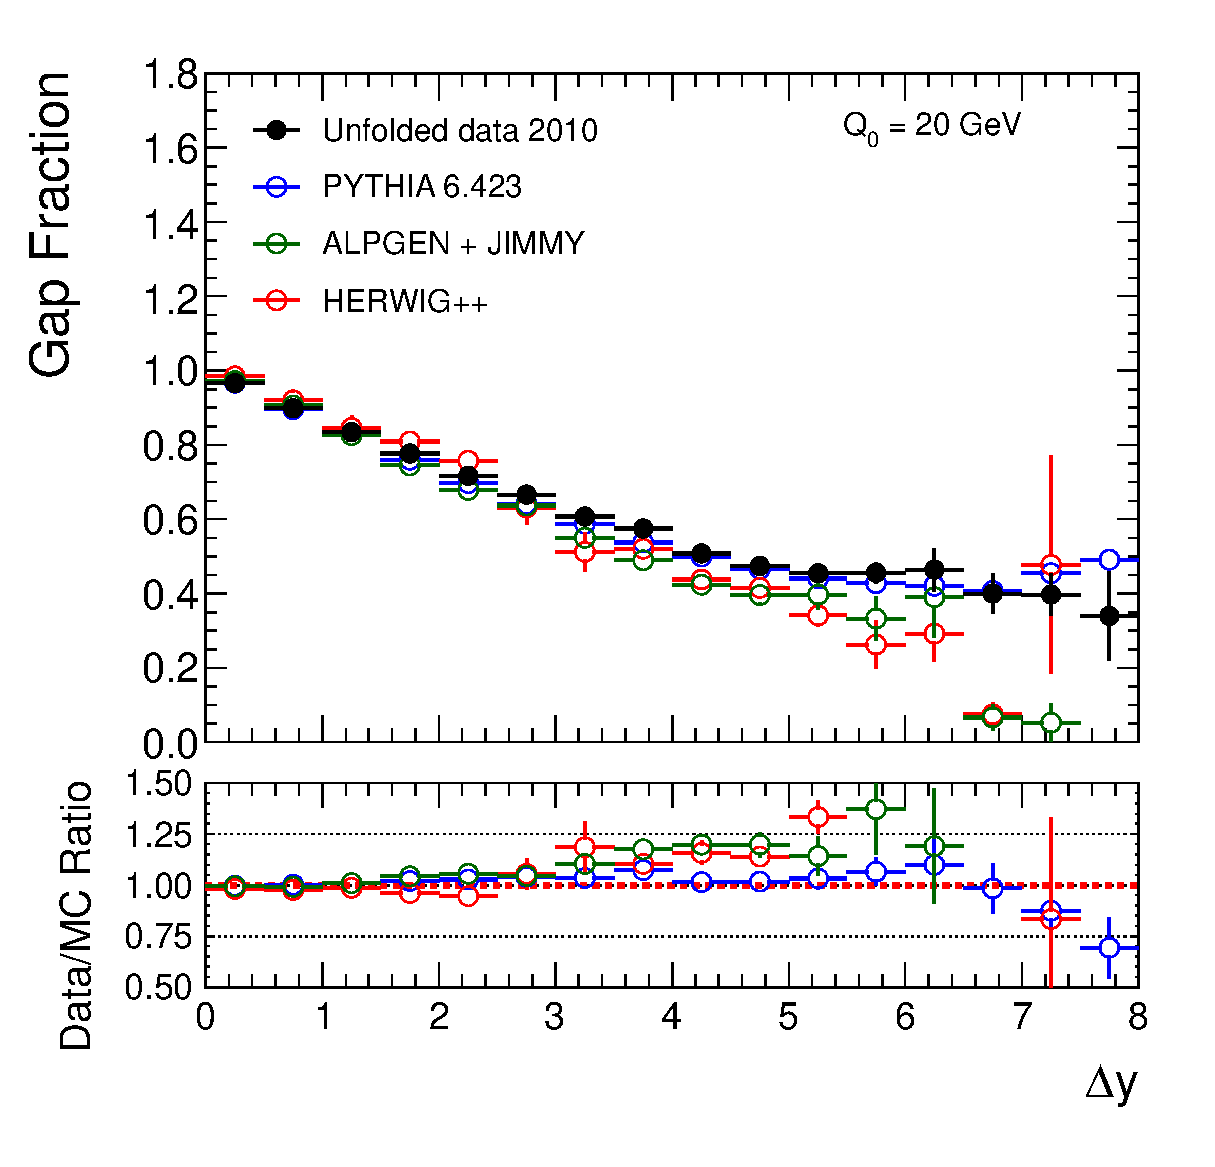
\includegraphics[width=\smallfigwidth]{chapters/azimuthal-decorrelation/GapFraction.dYBins.eps}
    \label{fig:azimuthal-decorrelation:gap_fraction_dY}}
  \quad
  \subfloat[Gap fraction as a function of \Qnought]{
    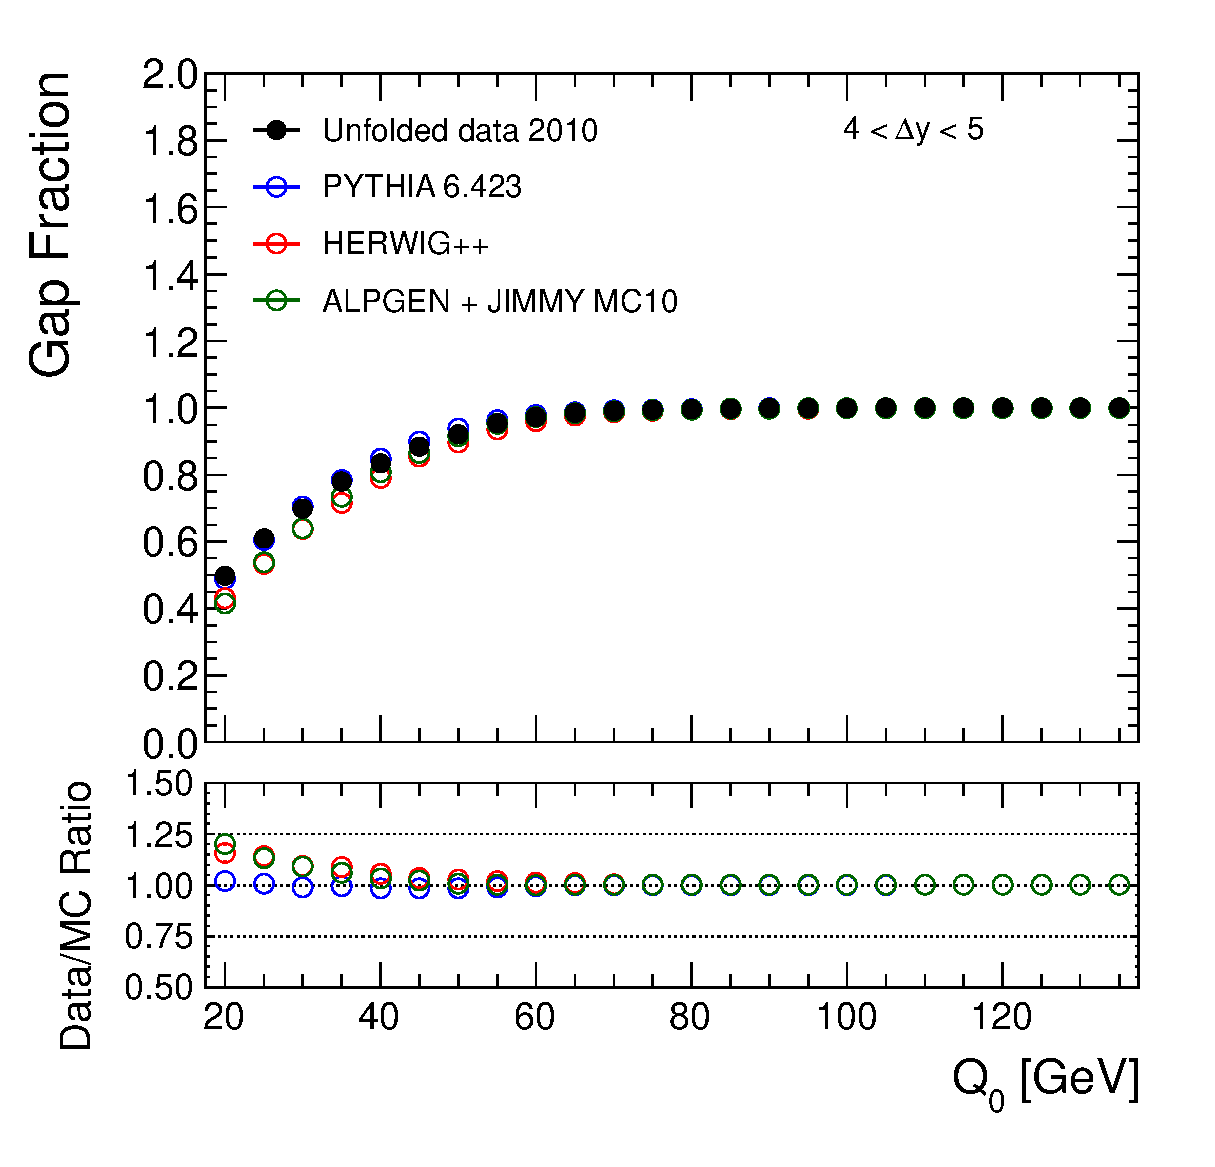
\includegraphics[width=\smallfigwidth]{chapters/azimuthal-decorrelation/GapFraction.4dY5.Q0Bins.eps}
    \label{fig:azimuthal-decorrelation:gap_fraction_Q0}}
  \caption{Gap fraction distributions as a function of \Qnought and \DeltaY for
           jets identified using the \akt algorithm with $R=0.6$. \protect\subref{fig:azimuthal-decorrelation:gap_fraction_dY}
           shows the gap fraction as a function of \DeltaY for $\Qnought = \unit{20}{\GeV}$,
           while \protect\subref{fig:azimuthal-decorrelation:gap_fraction_Q0} shows the gap fraction as a function of \Qnought in the region
           $4 \leq \DeltaY < 5$. The unfolded data are compared to the leading order particle level \Pythia 6.423, \Herwigpp
           and \Alpgen predictions. The error bars indicate the statistical uncertainty
           on the measurement.}
  \label{fig:azimuthal-decorrelation:gap_fraction}
\end{figure}

\FigureRef{fig:azimuthal-decorrelation:cosDeltaPhi} shows the \meanCosDPhi and \meanCosTwoDPhi
distributions as a function of \DeltaY for both inclusive and gap events. In general, there
is good agreement between the data and the different \MC generators, with
the major areas of disagreement coming at high \DeltaY, where statistics are
poorer. These disagreements are only present in the inclusive sample; once the
jet veto is applied the different \MC predictions agree well.

\begin{figure}[htpb]
  \subfloat[\meanCosDPhi, inclusive events]{
    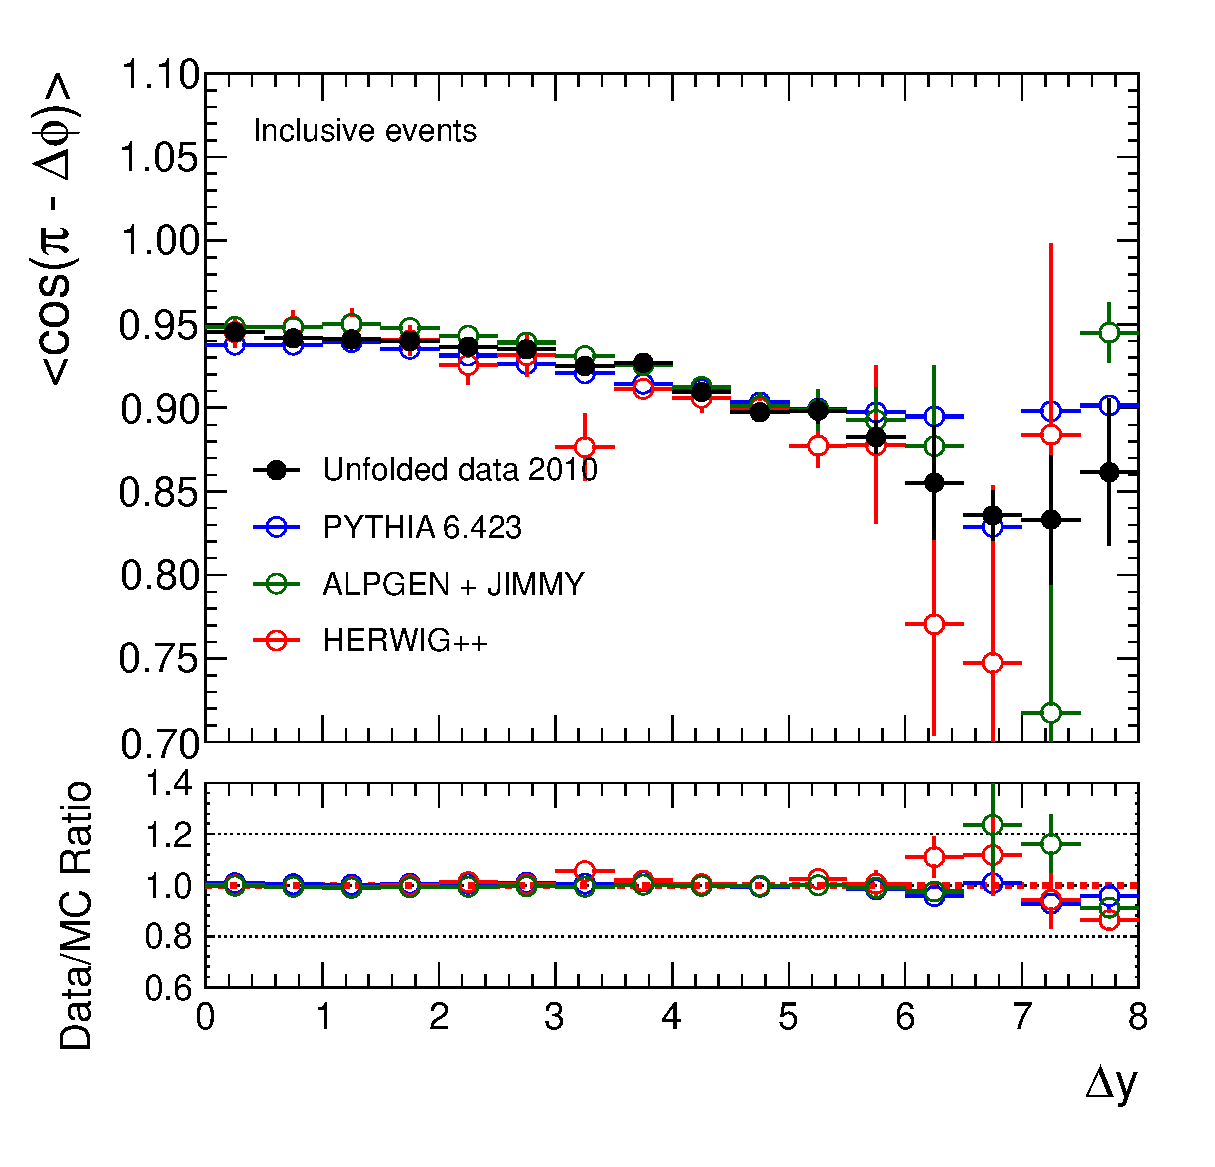
\includegraphics[width=\smallfigwidth]{chapters/azimuthal-decorrelation/Inclusive.CosDeltaPhi.dYBins.eps}
    \label{fig:azimuthal-decorrelation:cos_inclusive}}
  \quad
  \subfloat[\meanCosDPhi, gap events]{
    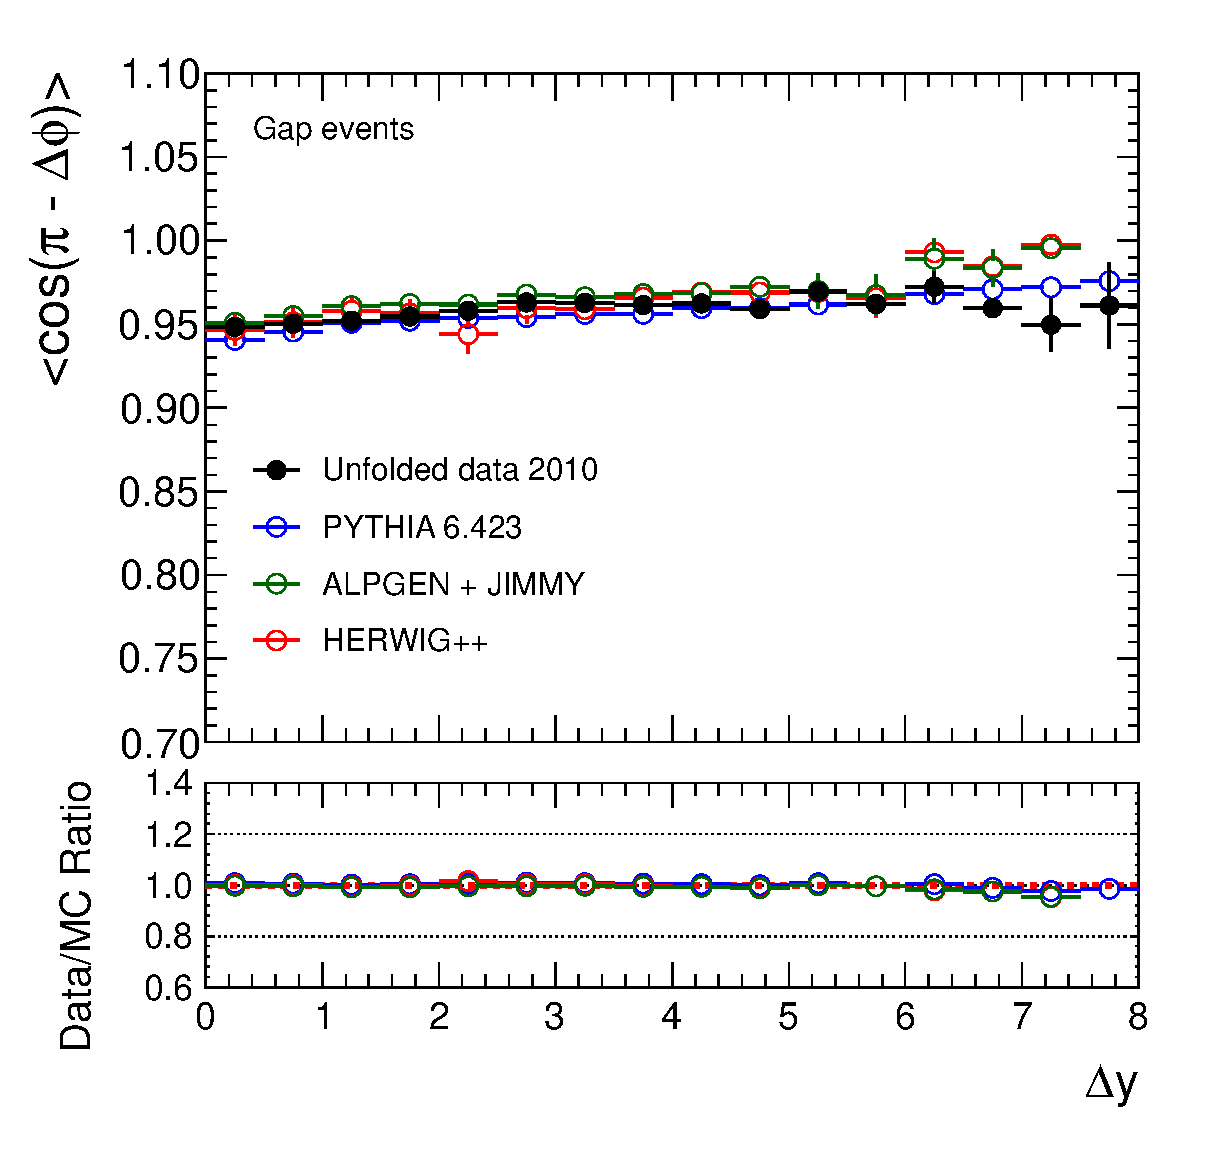
\includegraphics[width=\smallfigwidth]{chapters/azimuthal-decorrelation/Gap.CosDeltaPhi.dYBins.eps}
    \label{fig:azimuthal-decorrelation:cos_gap}}
  \\
  \subfloat[\meanCosTwoDPhi, inclusive events]{
    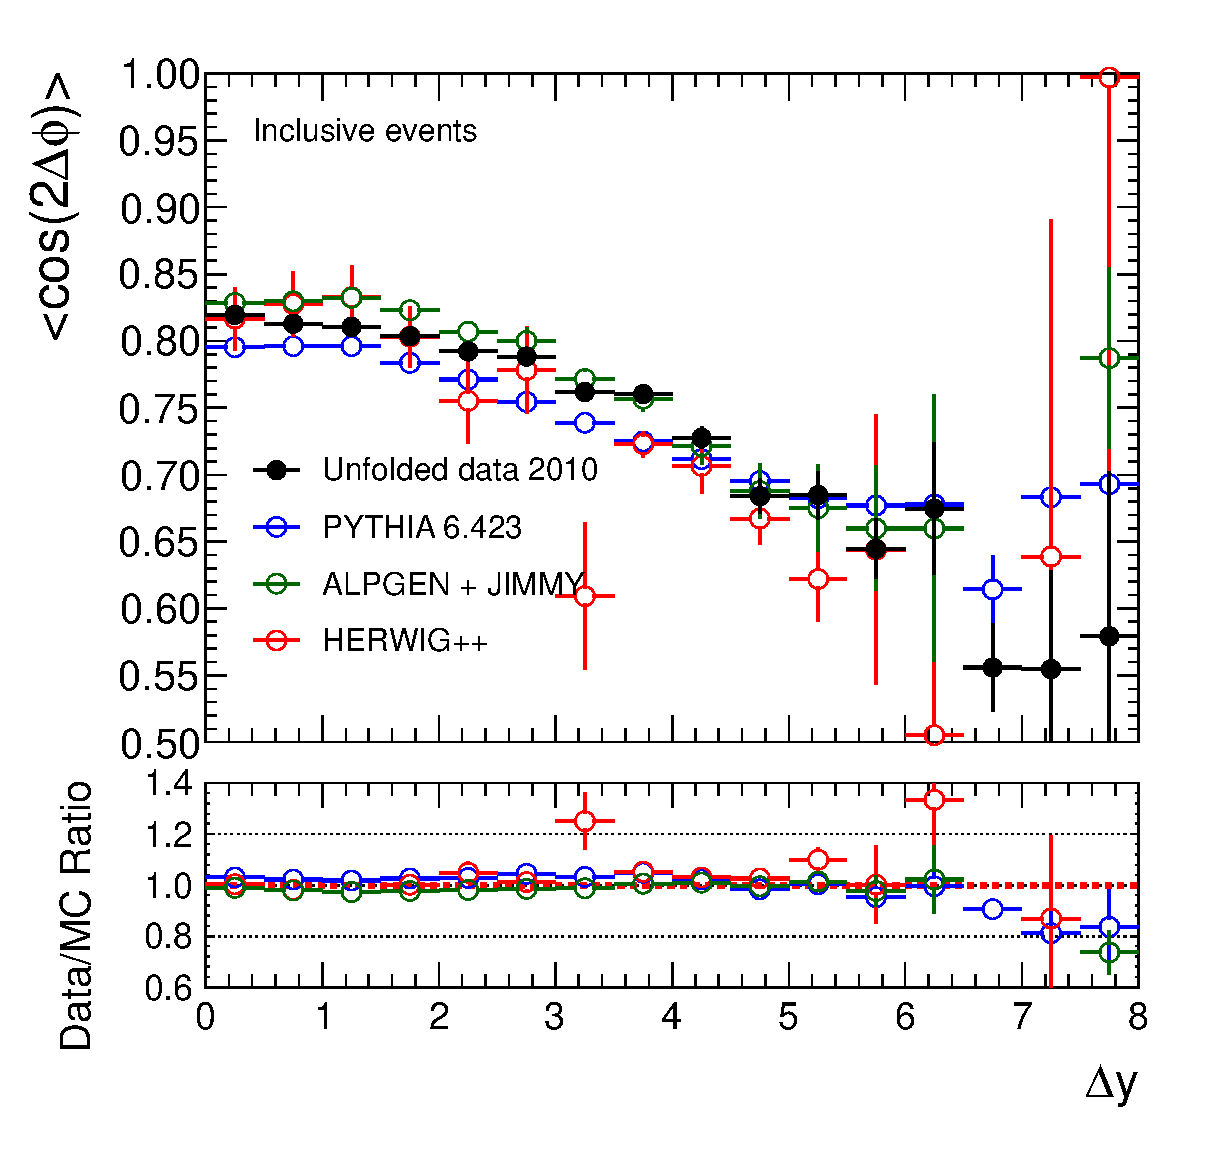
\includegraphics[width=\smallfigwidth]{chapters/azimuthal-decorrelation/Inclusive.CosTwoDeltaPhi.dYBins.eps}
    \label{fig:azimuthal-decorrelation:cosTwo_inclusive}}
  \quad
  \subfloat[\meanCosTwoDPhi, gap events]{
    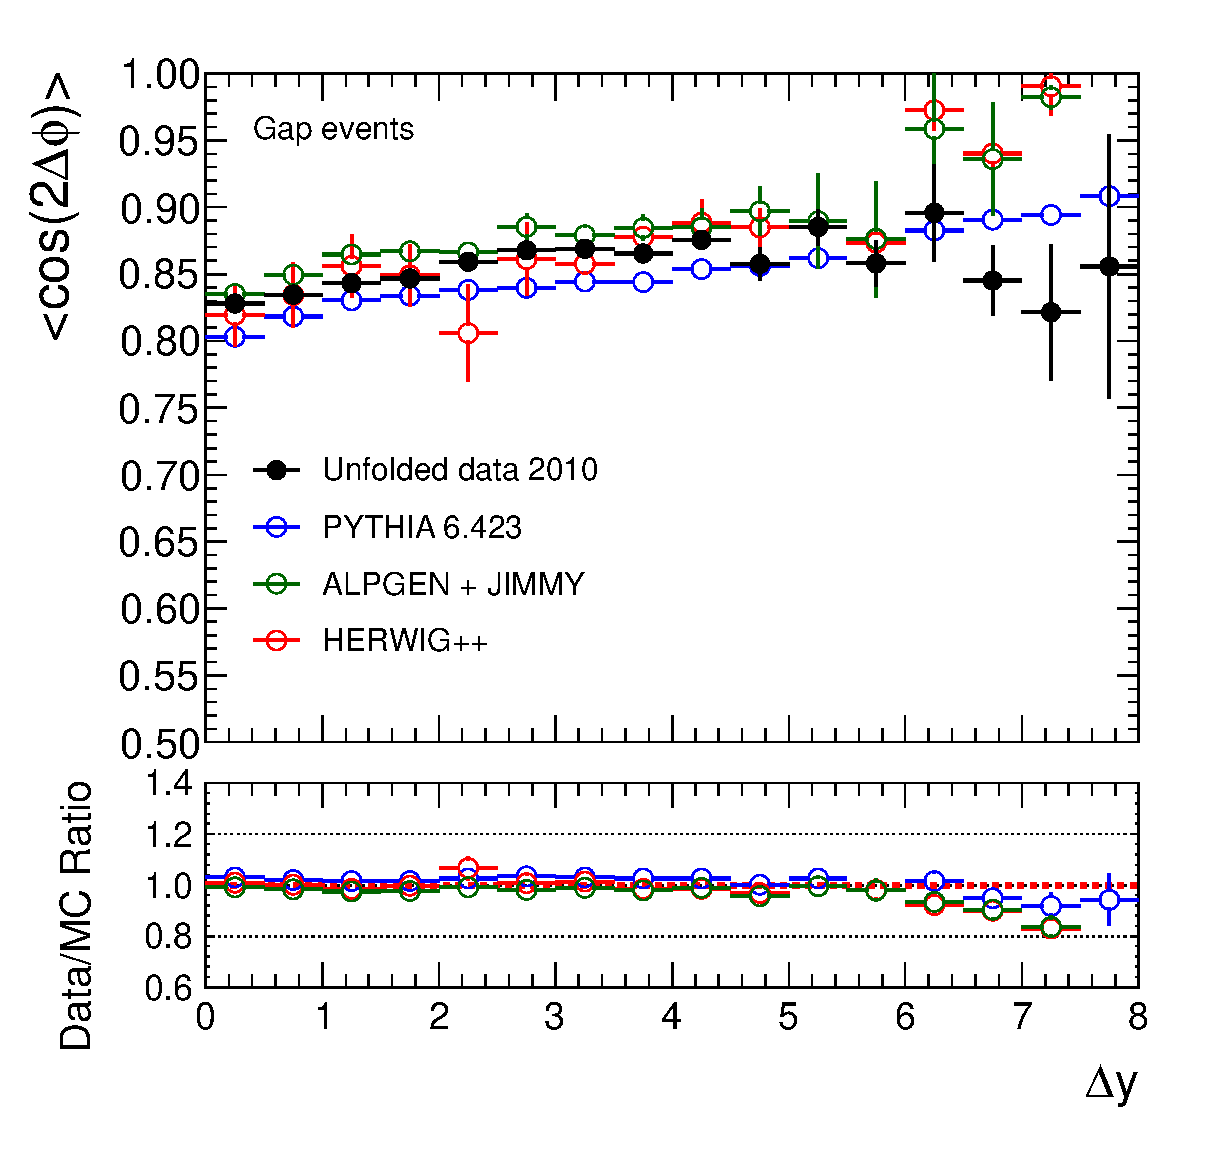
\includegraphics[width=\smallfigwidth]{chapters/azimuthal-decorrelation/Gap.CosTwoDeltaPhi.dYBins.eps}
    \label{fig:azimuthal-decorrelation:cosTwo_gap}}
  \caption{Distributions of \meanCosDPhi (top) and \meanCosTwoDPhi (bottom) shown as a function
           of \DeltaY for jets identified using the \akt algorithm with $R=0.6$.
           Inclusive events (left) and gap events (right) are shown separately.
           The unfolded data are compared to the leading order particle level \Pythia 6.423, \Herwigpp and \Alpgen predictions.
           The error bars indicate the statistical uncertainty on the measurement.}
  \label{fig:azimuthal-decorrelation:cosDeltaPhi}
\end{figure}

Figures~\ref{fig:azimuthal-decorrelation:cross-sections_dPhi},~\ref{fig:azimuthal-decorrelation:cross-sections_cosDPhi}~and~\ref{fig:azimuthal-decorrelation:cross-sections_cosTwoDPhi}
show the \DeltaPhi, \cosDPhi and \cosTwoDPhi \xs{s} respectively, for six different
\DeltaY bins. Inclusive events and gap events are shown separately. Only
comparison between \Pythia and data is shown here, since the other leading
order \MC generators suffer from poor statistics at large \DeltaY. Bins in which
only a single event is present have been removed from these plots.
%Agreement between the data and both \Pythia and
%\Herwig is reasonably close, especially since these are leading order \MC
%generators. Agreement with \Alpgen is less good, suffering from limited
%statistics, particularly at large \DeltaY.

\begin{figure}[htpb]
  \subfloat[\Xs as a function of \DeltaPhi for inclusive events]{
    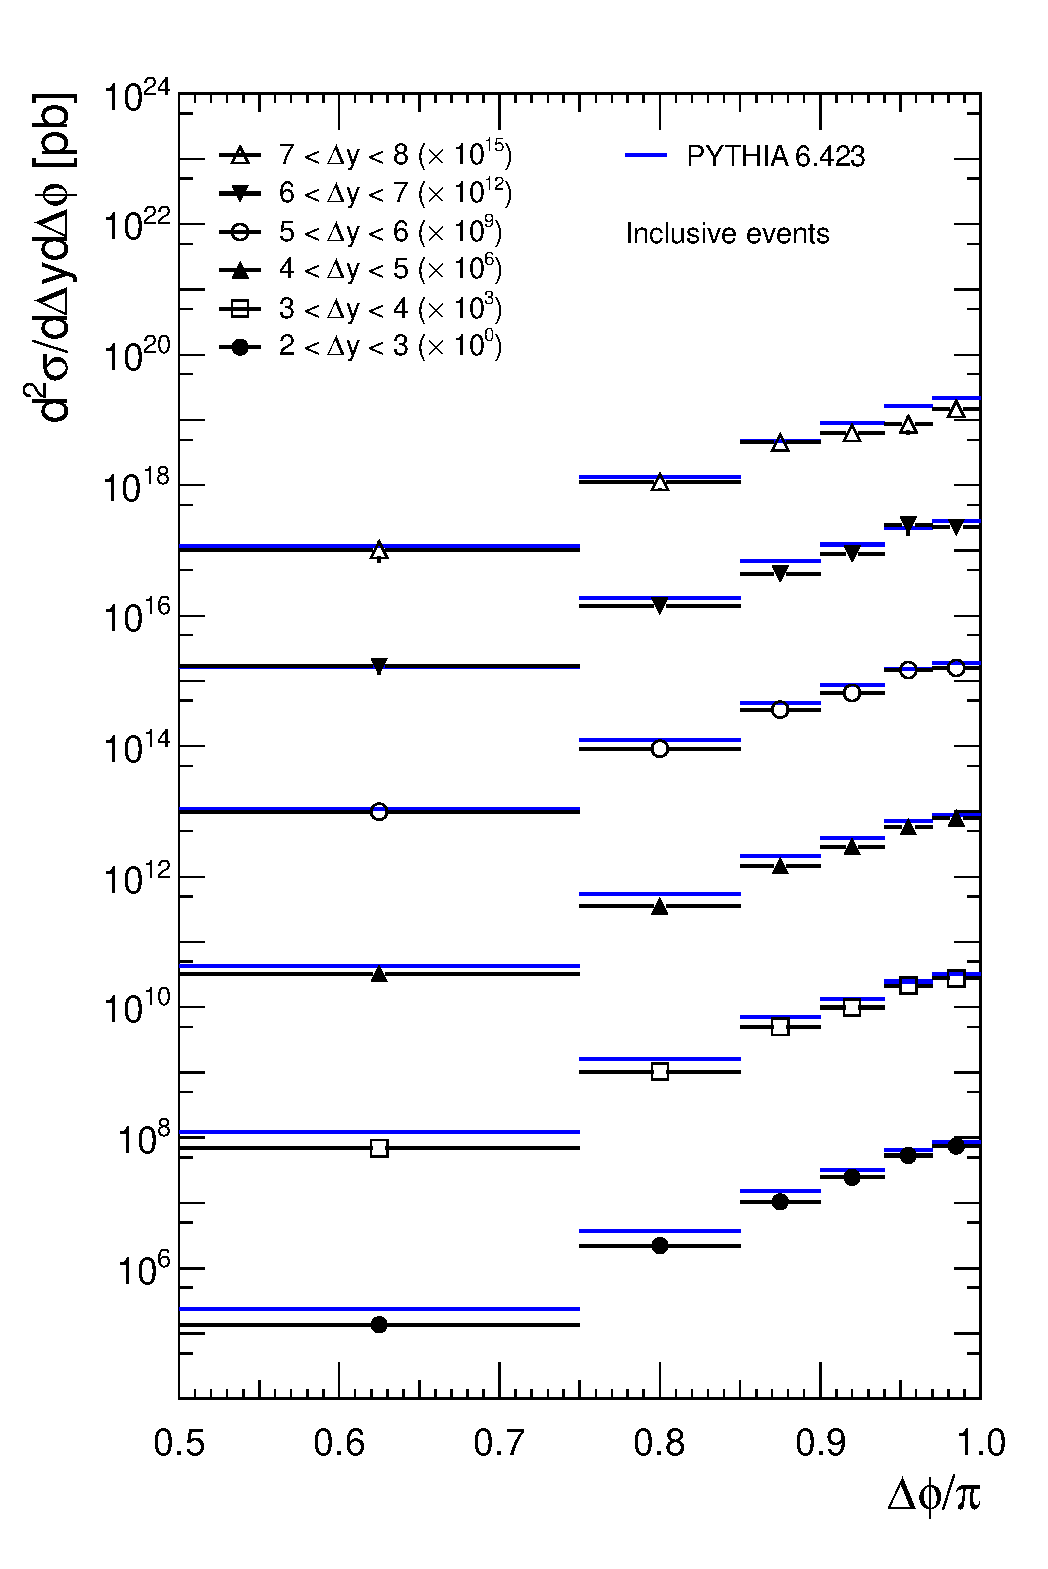
\includegraphics[width=\smallfigwidth]{chapters/azimuthal-decorrelation/Inclusive.CrossSection.all_dY_slices.dPhiBins.eps}
    \label{fig:azimuthal-decorrelation:cross-section_DeltaPhi_inclusive}}
  \quad
  \subfloat[\Xs as a function of \DeltaPhi for gap events]{
    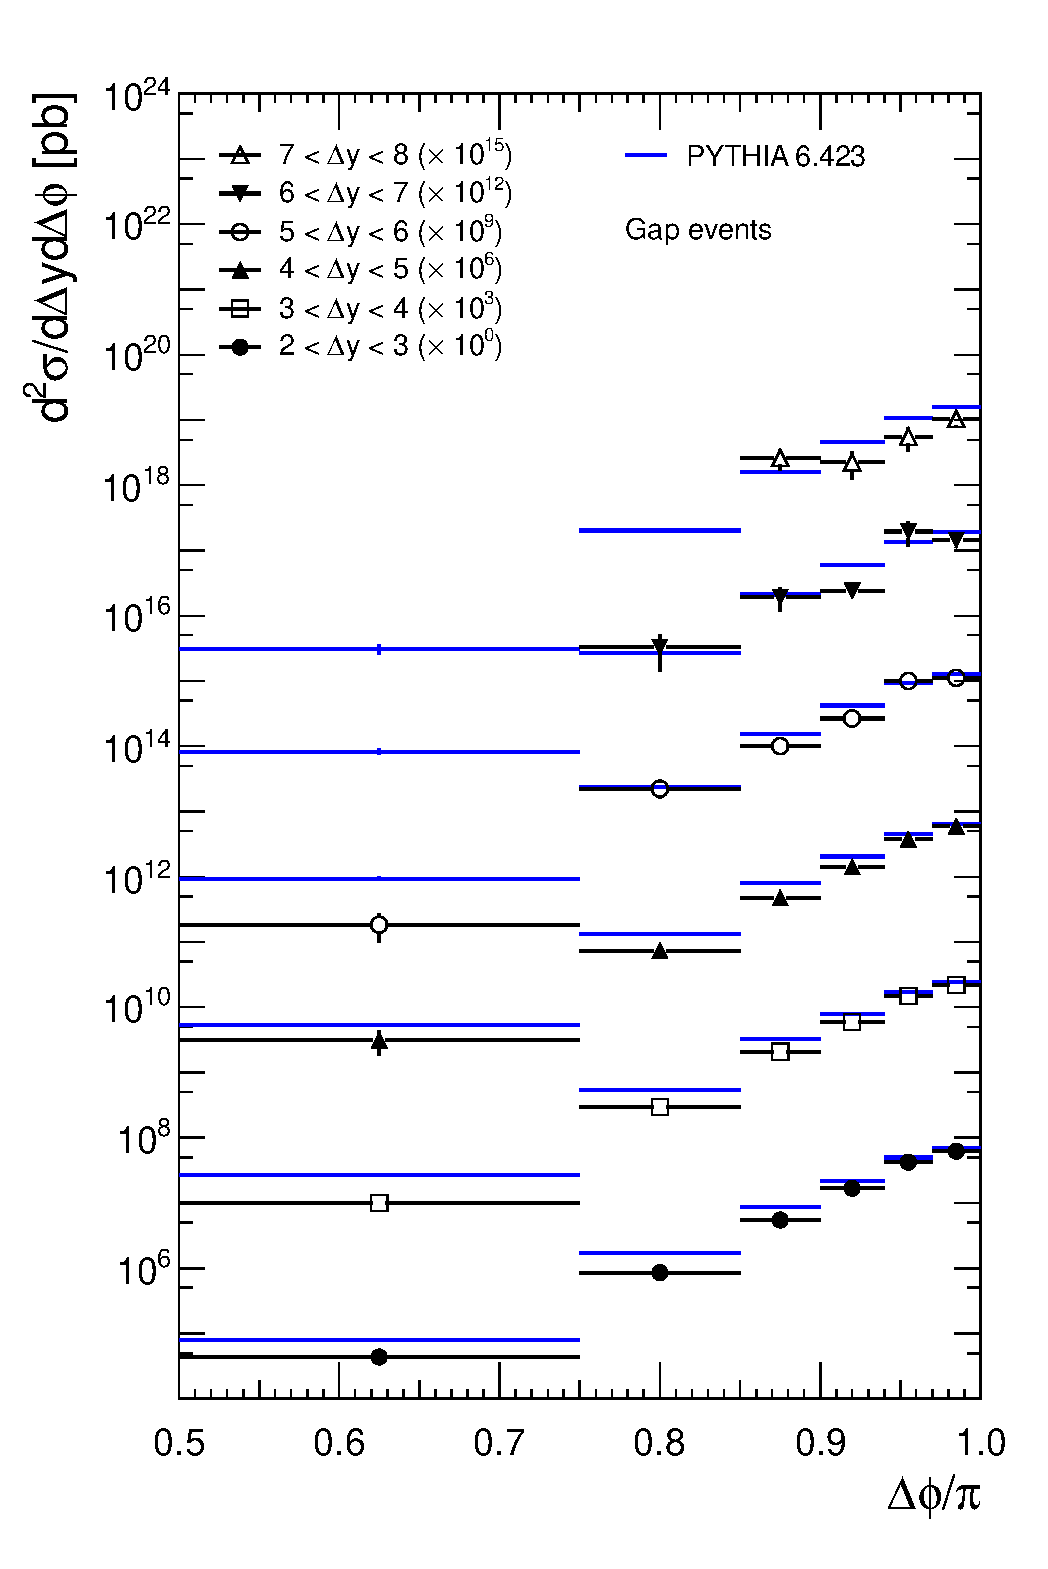
\includegraphics[width=\smallfigwidth]{chapters/azimuthal-decorrelation/Gap.CrossSection.all_dY_slices.dPhiBins.eps}
    \label{fig:azimuthal-decorrelation:cross-section_DeltaPhi_gap}}
  \caption{Double-differential \xs as a function of \DeltaPhi in different regions of \DeltaY.
           The \xs is shown for jets identified using the \akt algorithm with
           $R=0.6$. \protect\subref{fig:azimuthal-decorrelation:cross-section_DeltaPhi_inclusive}
           shows inclusive events while \protect\subref{fig:azimuthal-decorrelation:cross-section_DeltaPhi_gap}
           shows gap events. The unfolded data are compared to the leading order particle
           level \Pythia 6.423 prediction. In each case, the error bars
           indicate the statistical uncertainty on the measurement only. Statistically
           insignificant data points at large \DeltaY are omitted.}
  \label{fig:azimuthal-decorrelation:cross-sections_dPhi}
\end{figure}

\begin{figure}[htpb]
  \subfloat[\Xs as a function of \cosDPhi for inclusive events]{
    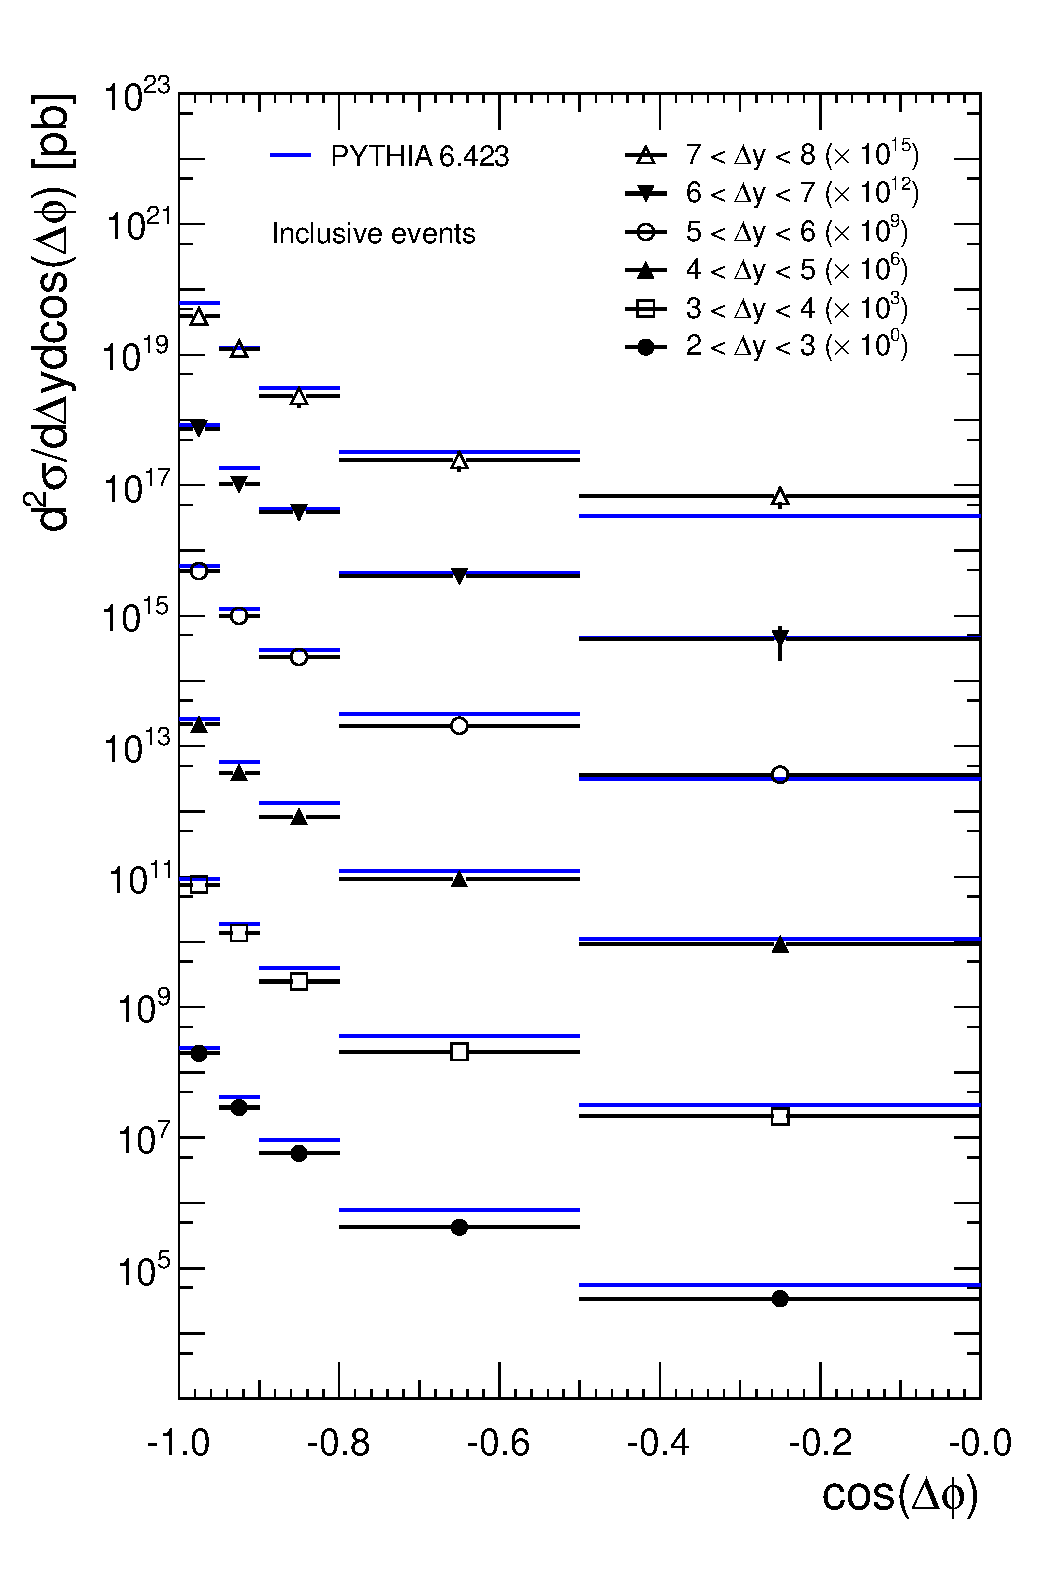
\includegraphics[width=\smallfigwidth]{chapters/azimuthal-decorrelation/Inclusive.CrossSection.all_dy_slices.CosDeltaPhiBins.eps}
    \label{fig:azimuthal-decorrelation:cross-section_CosDeltaPhi_inclusive}}
  \quad
  \subfloat[\Xs as a function of \cosDPhi for gap events]{
    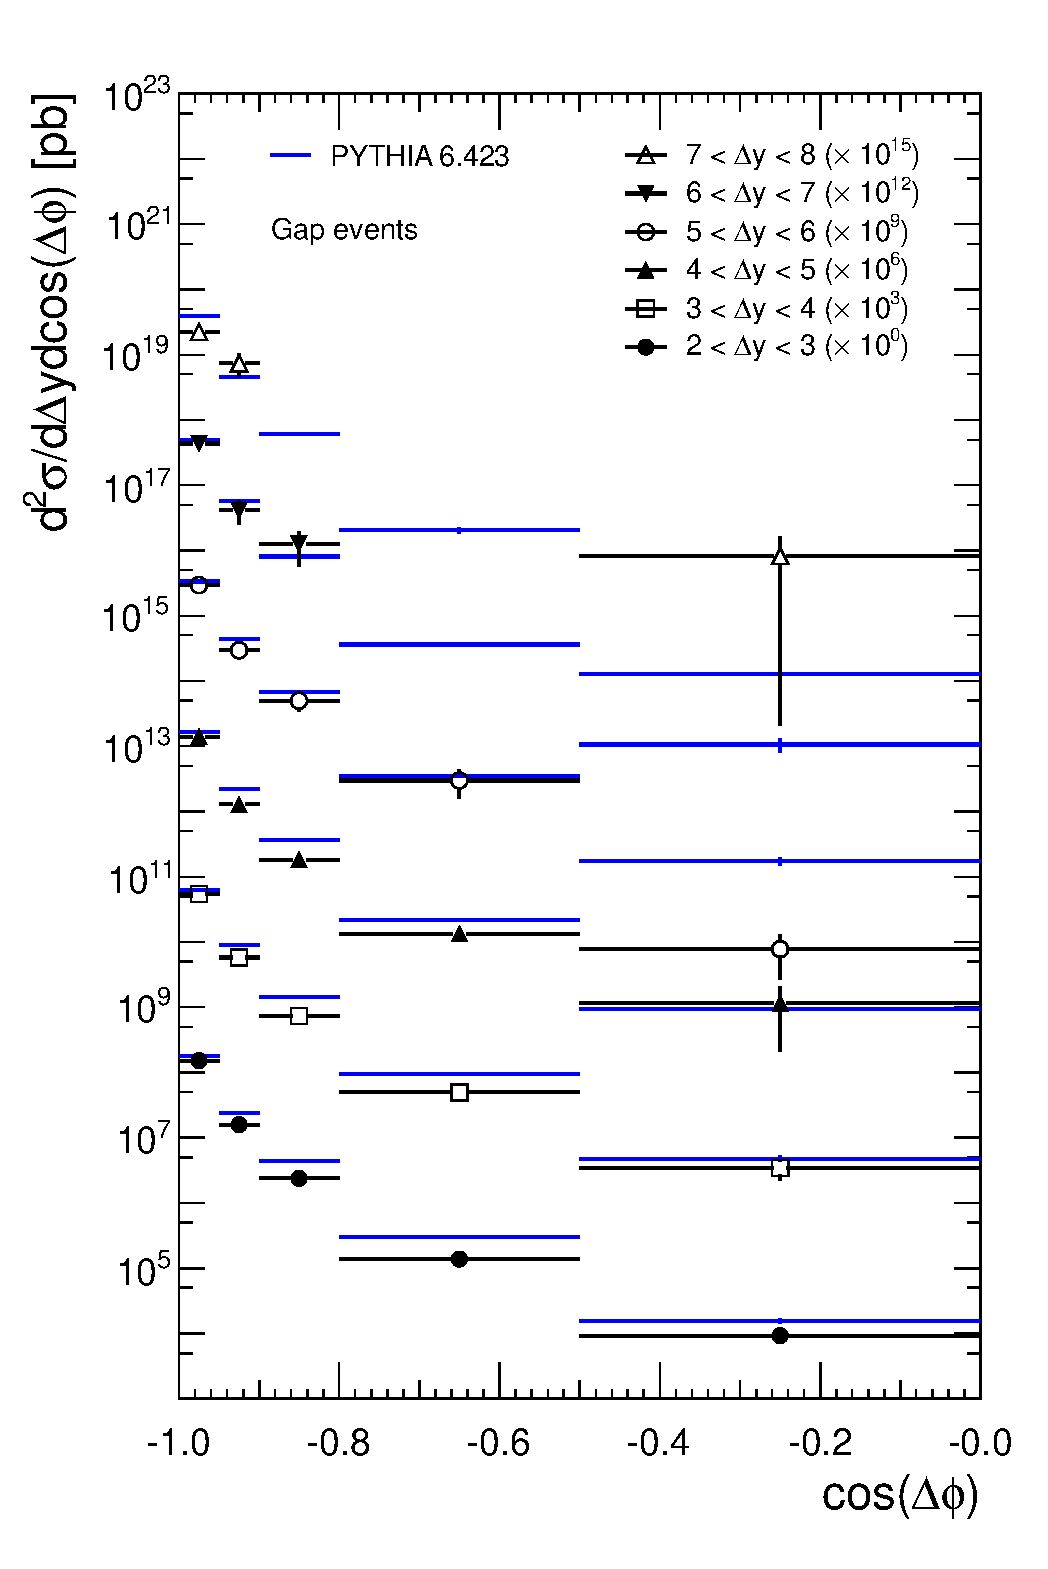
\includegraphics[width=\smallfigwidth]{chapters/azimuthal-decorrelation/Gap.CrossSection.all_dy_slices.CosDeltaPhiBins.eps}
    \label{fig:azimuthal-decorrelation:cross-section_CosDeltaPhi_gap}}
  \caption{Double-differential \xs as a function of \cosDPhi in different regions of \DeltaY.
           The \xs is shown for jets identified using the \akt algorithm with
           $R=0.6$. \protect\subref{fig:azimuthal-decorrelation:cross-section_CosDeltaPhi_inclusive}
           shows inclusive events, while \protect\subref{fig:azimuthal-decorrelation:cross-section_CosDeltaPhi_gap}
           shows gap events. The unfolded data are compared to the leading order particle
           level \Pythia 6.423 prediction. In each case, the error bars
           indicate the statistical uncertainty on the measurement only. Statistically
           insignificant data points at large \DeltaY are omitted.}
  \label{fig:azimuthal-decorrelation:cross-sections_cosDPhi}
\end{figure}

\begin{figure}[htpb]
  \subfloat[\Xs as a function of \cosTwoDPhi for inclusive events]{
    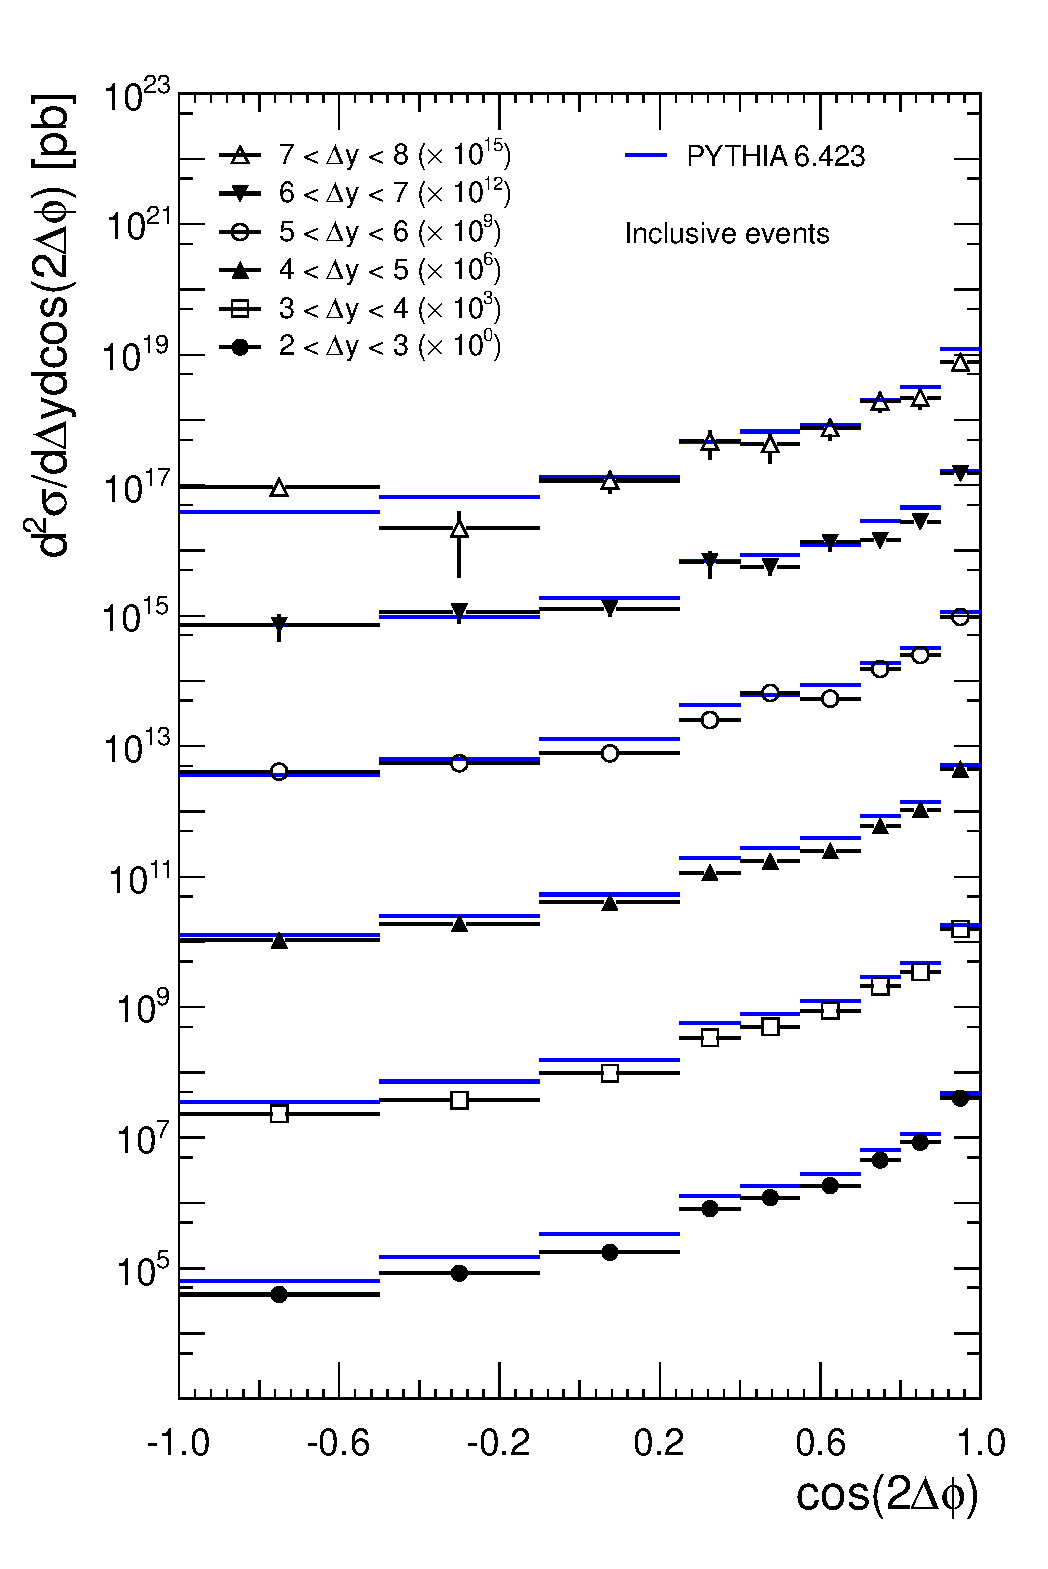
\includegraphics[width=\smallfigwidth]{chapters/azimuthal-decorrelation/Inclusive.CrossSection.all_dy_slices.CosTwoDeltaPhiBins.eps}
    \label{fig:azimuthal-decorrelation:cross-section_CosTwoDeltaPhi_inclusive}}
  \quad
  \subfloat[\Xs as a function of \cosTwoDPhi for gap events]{
    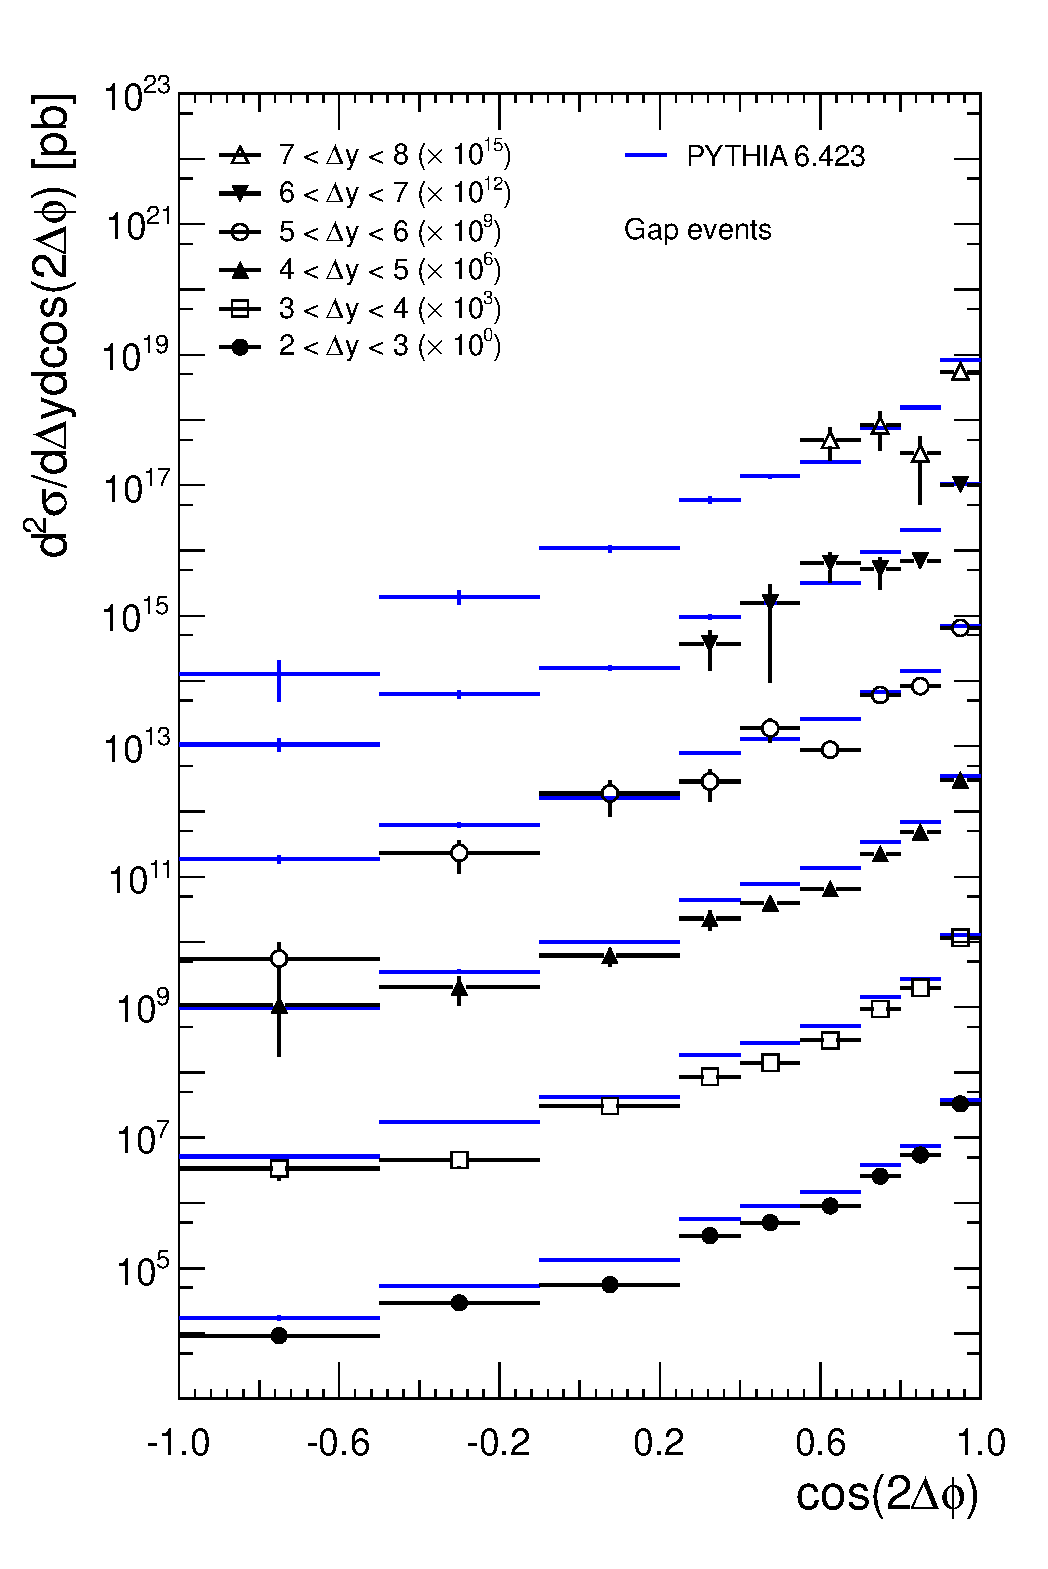
\includegraphics[width=\smallfigwidth]{chapters/azimuthal-decorrelation/Gap.CrossSection.all_dy_slices.CosTwoDeltaPhiBins.eps}
    \label{fig:azimuthal-decorrelation:cross-section_CosTwoDeltaPhi_gap}}
  \caption{Double-differential \xs as a function of \cosTwoDPhi in different regions of \DeltaY.
           The \xs is shown for jets identified using the \akt algorithm with
           $R=0.6$. \protect\subref{fig:azimuthal-decorrelation:cross-section_CosTwoDeltaPhi_inclusive}
           shows inclusive events, while \protect\subref{fig:azimuthal-decorrelation:cross-section_CosTwoDeltaPhi_gap}
           shows gap events. The unfolded data are compared to the leading order particle
           level \Pythia 6.423 prediction. In each case, the error bars
           indicate the statistical uncertainty on the measurement only. Statistically
           insignificant data points at large \DeltaY are omitted.}
  \label{fig:azimuthal-decorrelation:cross-sections_cosTwoDPhi}
\end{figure}

Finally, the distribution of number of jets in the gap, as a function of \DeltaY,
is shown in \FigureRef{fig:azimuthal-decorrelation:nGapJets}. Here, divergences
from the leading order \MC predictions can be seen at high \DeltaY, although \Pythia
still provides the best agreement with the data.

\begin{figure}
  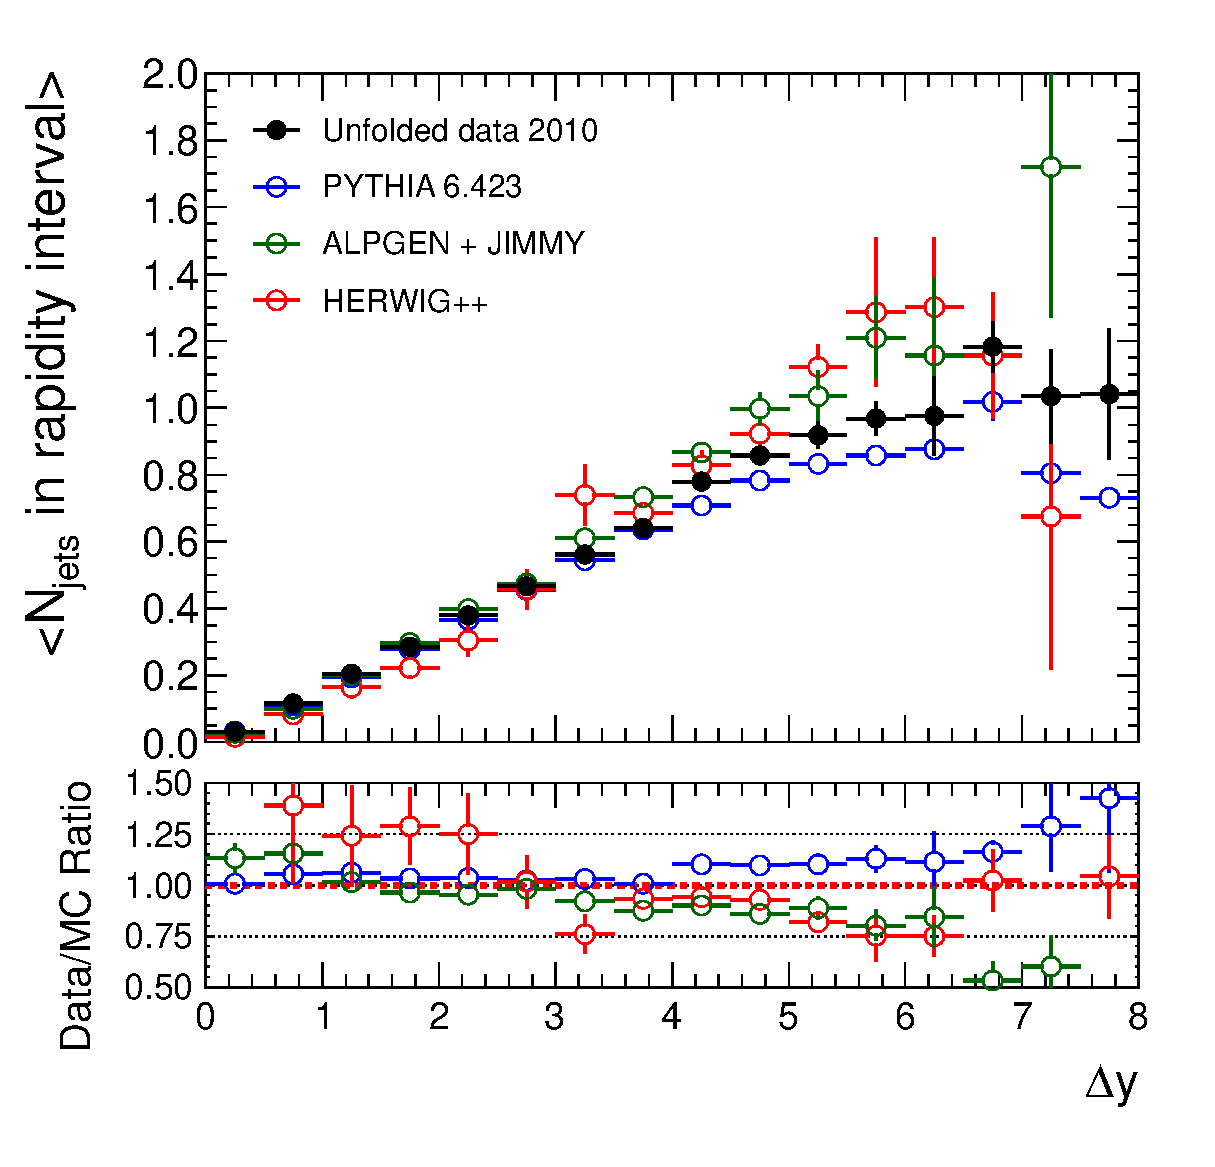
\includegraphics[width=\mediumfigwidth]{chapters/azimuthal-decorrelation/nGapJets.dYBins.eps}
  \caption{Mean number of jets in the gap as a function of \DeltaY. The veto scale
           is set to $\Qnought = \unit{20}{\GeV}$. The unfolded data are compared
           to the leading order particle level \Pythia 6.423, \Herwigpp and \Alpgen
           predictions. In each case, the error bars indicate the statistical uncertainty
           on the measurement only.}
  \label{fig:azimuthal-decorrelation:nGapJets}
\end{figure}

\subsection{Comparison to Higher Order \MC Generators}
Preliminary predictions from next-to-leading order generators are shown here, using
the MSTW2008 PDF set in all cases. Unfolded data are compared against \HEJ interfaced
with the \Ariadne parton shower~\cite{Lonnblad:1992:Ariadne}, \Powheg showered with
\Pythia and \Powheg showered with \Herwig; the same particle level events are used
for both of these \Powheg predictions. For the data, the errors shown reflect
statistical uncertainties, with systematic uncertainties arising from the effects
of jet energy scale, jet resolution and \DeltaPhi pointing resolution added in quadrature;
uncertainties arising from the unfolding procedure have not yet been evaluated.
For \Powheg, statistical uncertainties are combined with scale uncertainties, evaluated
by varying the renormalisation and factorisation scales by factors of two in each
direction; \HEJ shows only the statistical uncertainties.

\FigureRef{fig:azimuthal-decorrelation:gap_fraction_theory} shows the gap fraction
as a  function of \DeltaY and as a function of \Qnought for three different \DeltaY
slices. Large divergences between the \MC predictions can be seen throughout, these
are accentuated at high \DeltaY. The best agreement with the data comes from the
\Powheg+\Pythia prediction, although even this shows large levels of disagreement
as \DeltaY increases.

\begin{figure}[htpb]
  \subfloat[Gap fraction as a function of \DeltaY]{
    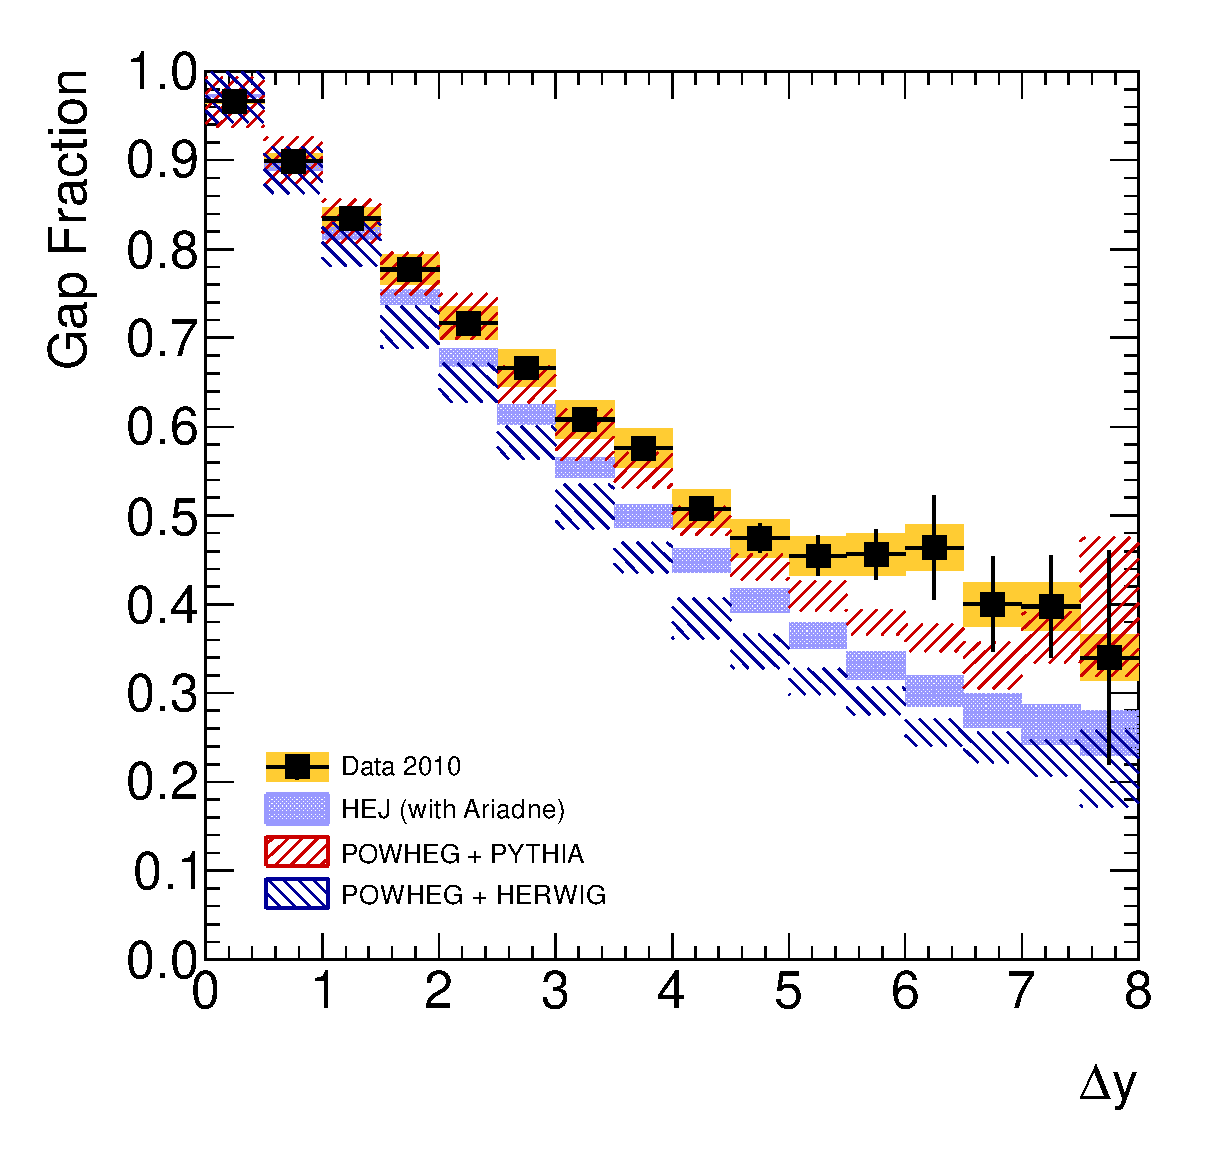
\includegraphics[width=\smallfigwidth]{chapters/azimuthal-decorrelation/GapFraction_YDist.eps}
    \label{fig:azimuthal-decorrelation:gap_fraction_dY_theory}}
  \quad
  \subfloat[Gap fraction as a function of \Qnought]{
    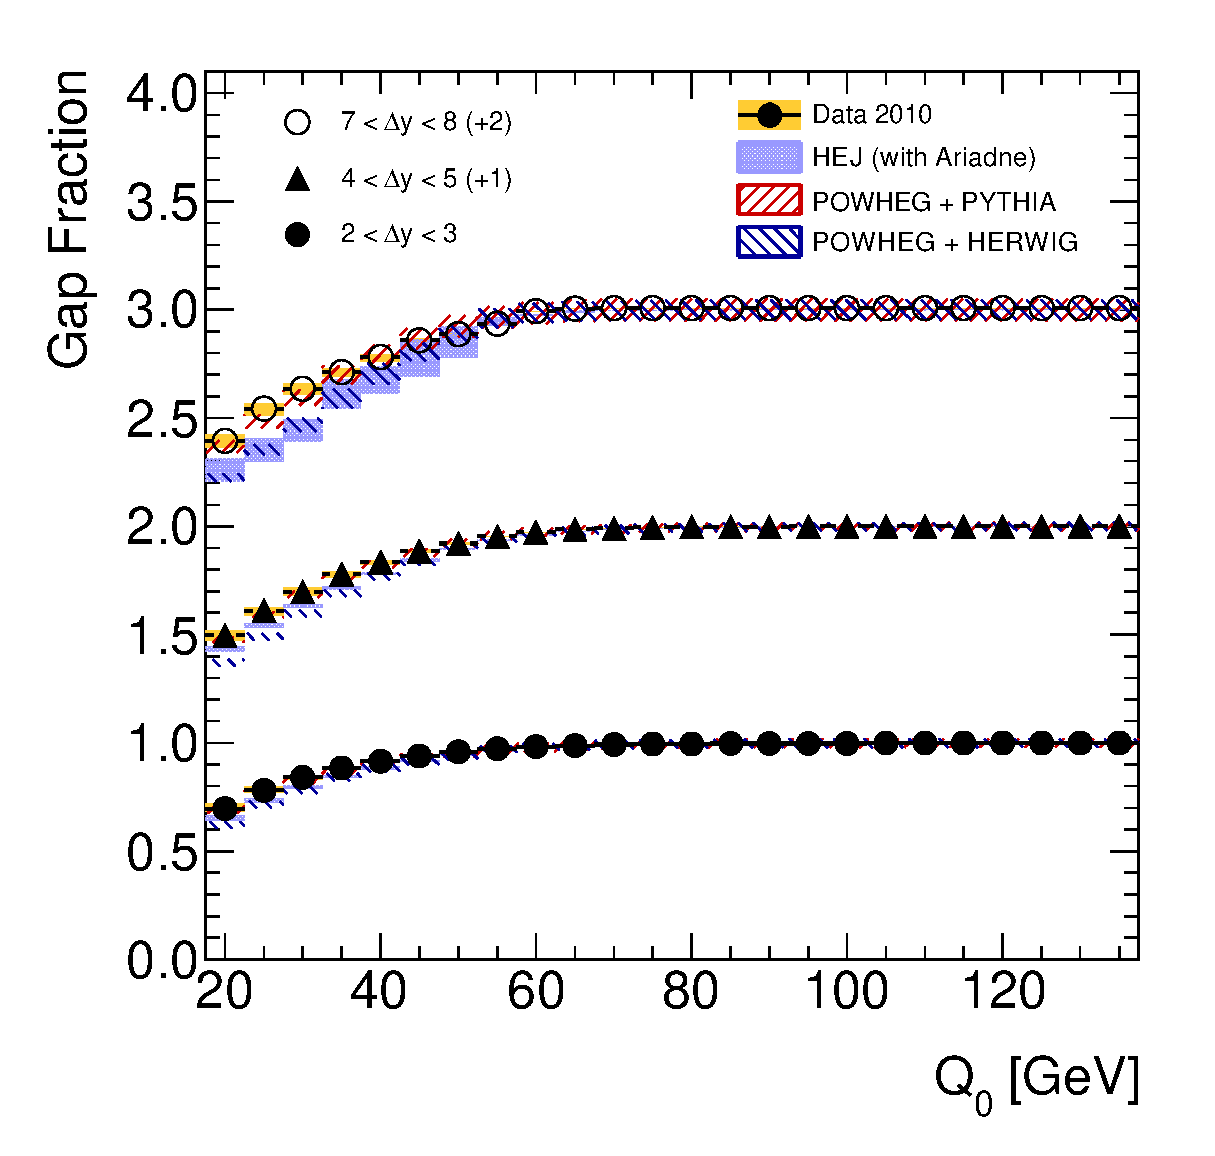
\includegraphics[width=\smallfigwidth]{chapters/azimuthal-decorrelation/GapFraction_Q0.eps}
    \label{fig:azimuthal-decorrelation:gap_fraction_Q0_theory}}
  \caption{Gap fraction distributions as a function of \Qnought and \DeltaY for
           jets identified using the \akt algorithm with $R=0.6$. \protect\subref{fig:azimuthal-decorrelation:gap_fraction_dY_theory}
           shows the gap fraction as a function of \DeltaY for $\Qnought = \unit{20}{\GeV}$,
           while \protect\subref{fig:azimuthal-decorrelation:gap_fraction_Q0_theory} shows
           the gap fraction as a function of \Qnought for three different
           slices in \DeltaY. The unfolded data are compared to the \HEJ, \Powheg+\Pythia
           and \Powheg+\Herwig. The error bars on data indicate the statistical
           uncertainty on the measurement with a series of systematic uncertainties
           summarised by the orange band. The error bands on the \MC predictions
           represent the statistical errors only, in the case of \HEJ, with the
           scale uncertainties also combined in the case of \Powheg.}
  \label{fig:azimuthal-decorrelation:gap_fraction_theory}
\end{figure}

\FigureRef{fig:azimuthal-decorrelation:cosDeltaPhi_theory} shows the \meanCosDPhi and \meanCosTwoDPhi
distributions as a function of \DeltaY for both inclusive and gap events. In general, there
is good agreement between the data and the different \MC generators, with
the major areas of disagreement coming at high \DeltaY, where statistics are
poorer. These disagreements are only present in the inclusive sample; once the
jet veto is applied the different \MC predictions agree well.

\begin{figure}[htpb]
  \subfloat[\meanCosDPhi, inclusive events]{
    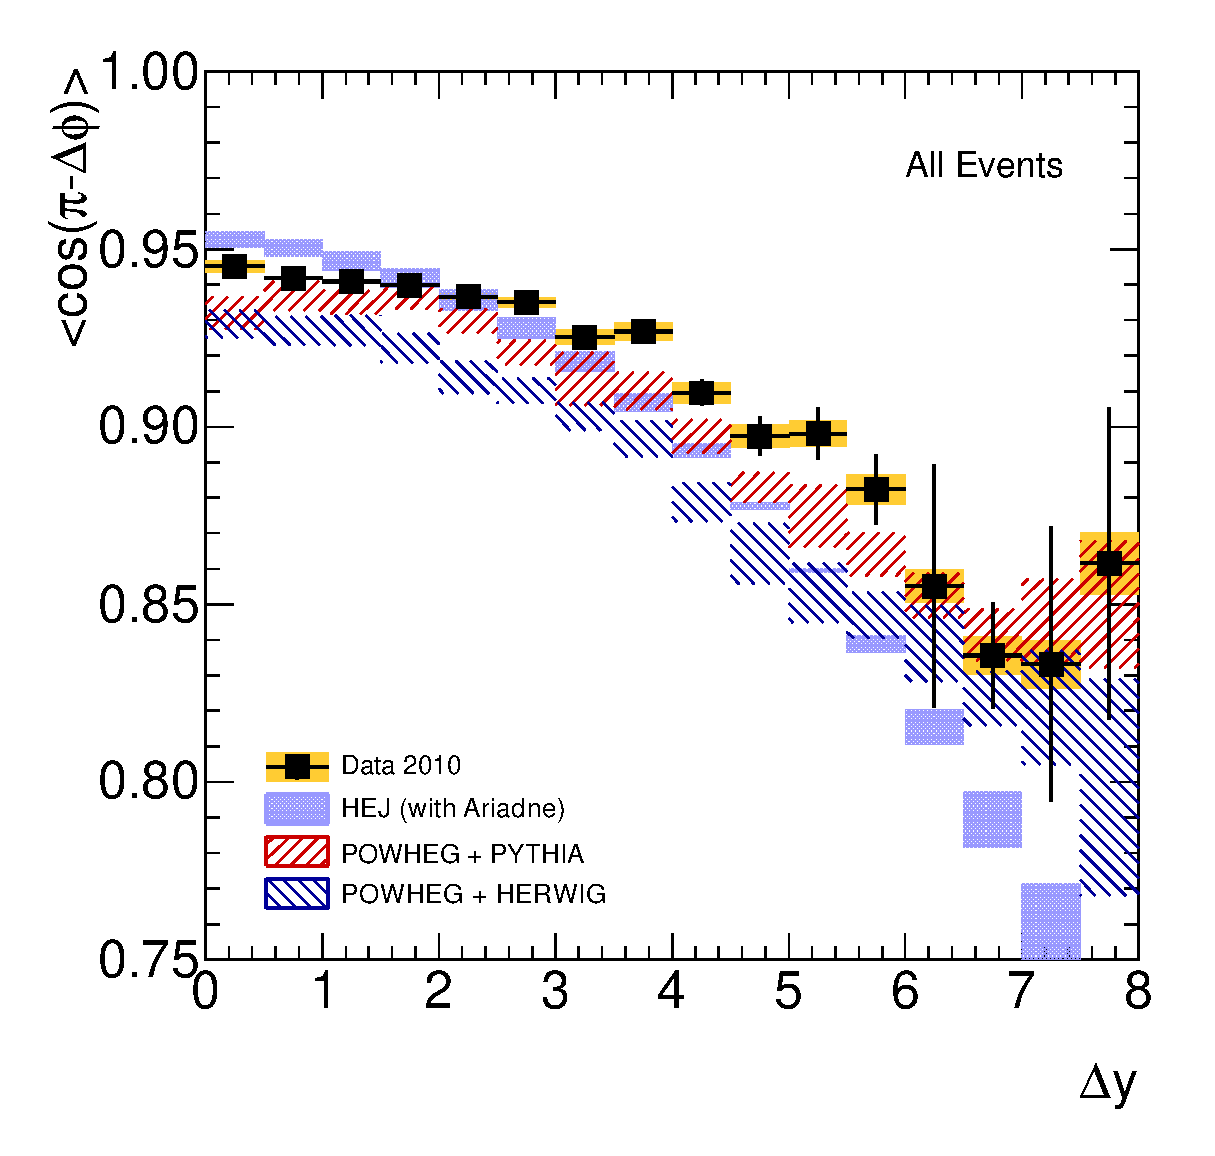
\includegraphics[width=\smallfigwidth]{chapters/azimuthal-decorrelation/CosDphiInclusive_YDist.eps}
    \label{fig:azimuthal-decorrelation:cos_inclusive_theory}}
  \quad
  \subfloat[\meanCosDPhi, gap events]{
    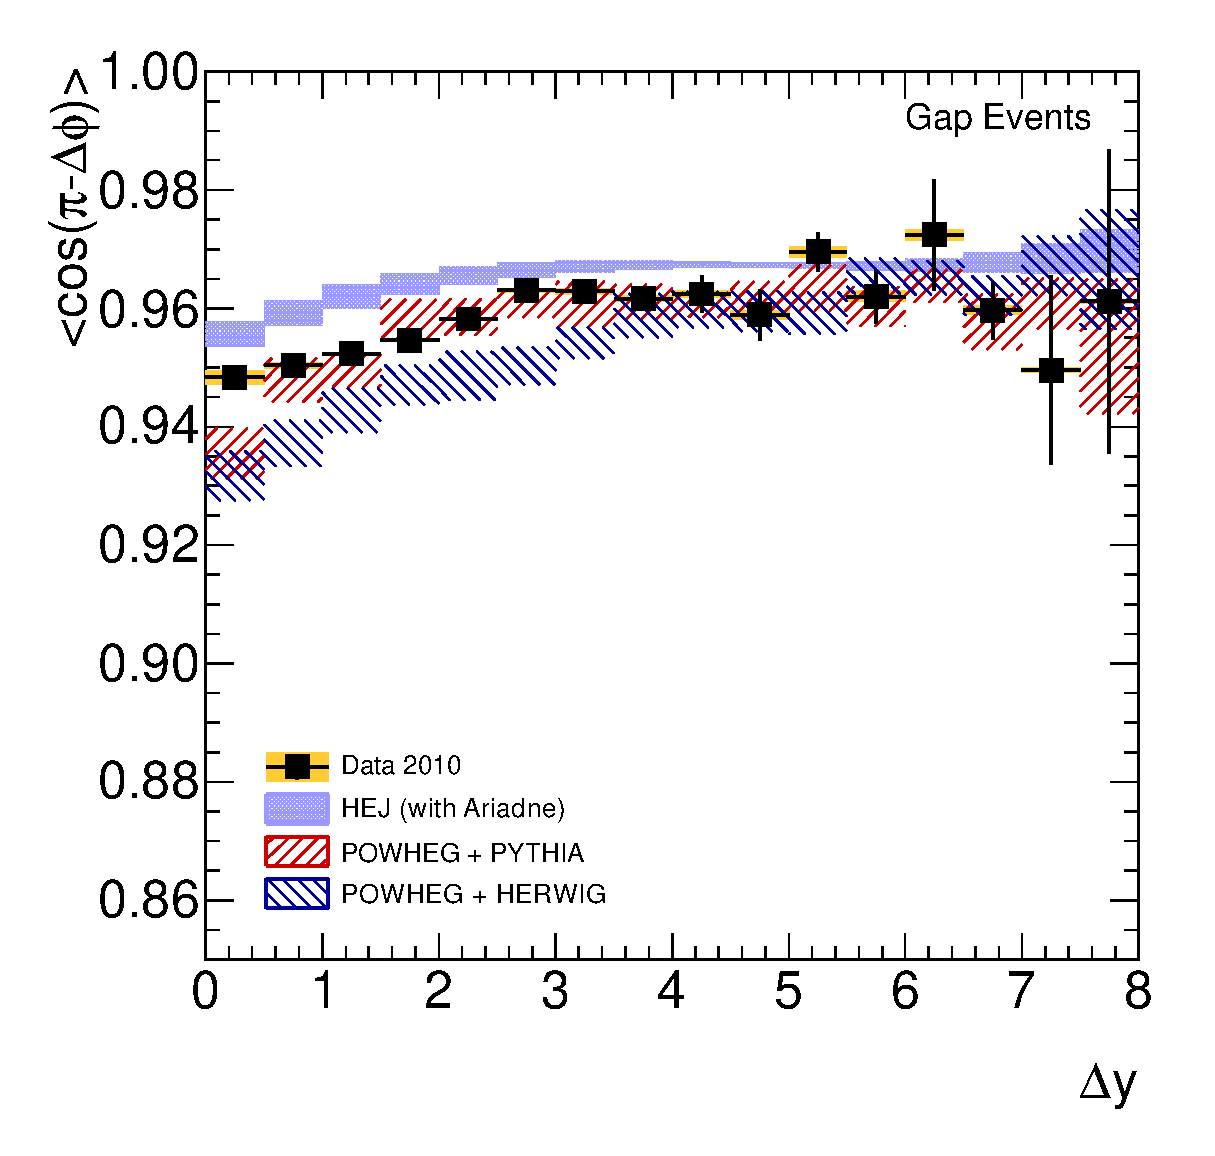
\includegraphics[width=\smallfigwidth]{chapters/azimuthal-decorrelation/CosDphiGap_YDist.eps}
    \label{fig:azimuthal-decorrelation:cos_gap_theory}}
  \\
  \subfloat[\meanCosTwoDPhi, inclusive events]{
    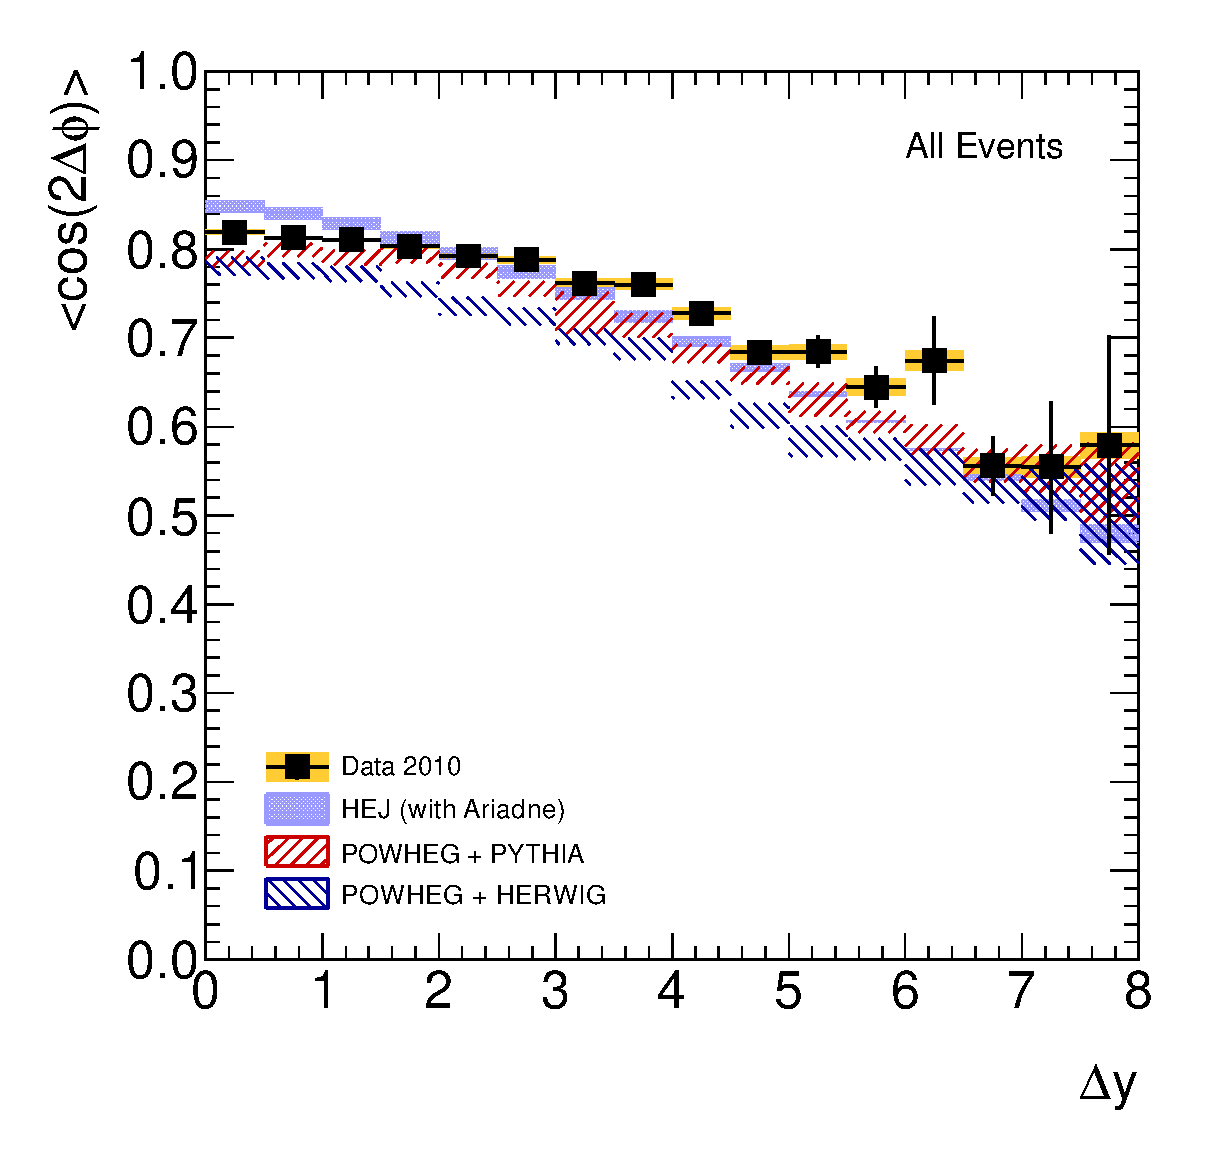
\includegraphics[width=\smallfigwidth]{chapters/azimuthal-decorrelation/CosTwoDphiInclusive_YDist.eps}
    \label{fig:azimuthal-decorrelation:cosTwo_inclusive_theory}}
  \quad
  \subfloat[\meanCosTwoDPhi, gap events]{
    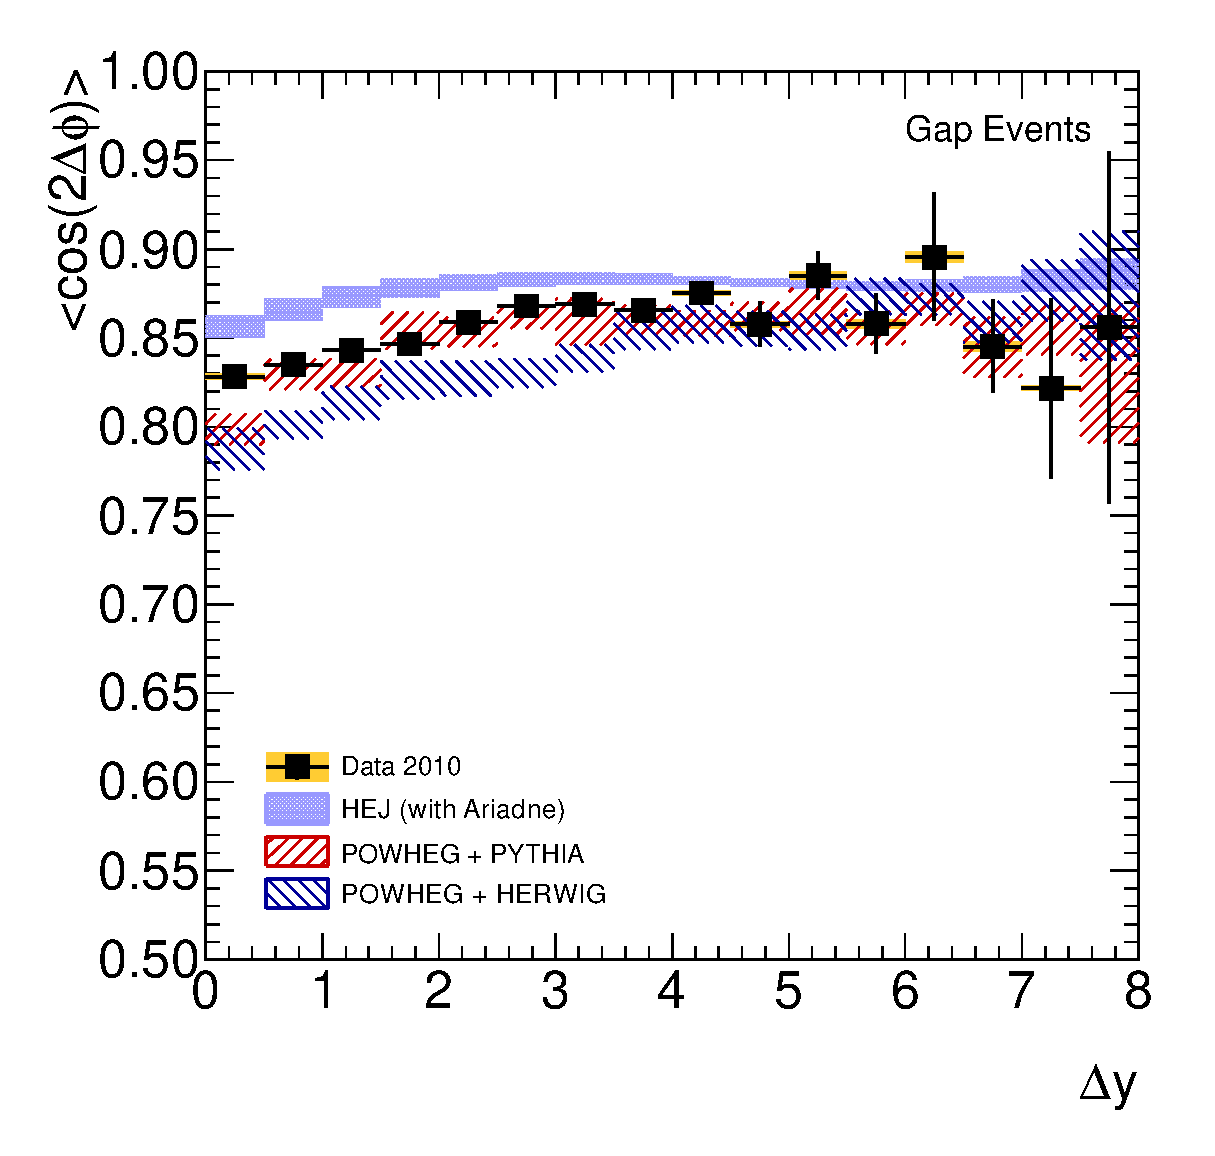
\includegraphics[width=\smallfigwidth]{chapters/azimuthal-decorrelation/CosTwoDphiGap_YDist.eps}
    \label{fig:azimuthal-decorrelation:cosTwo_gap_theory}}
  \caption{Distributions of \meanCosDPhi (top) and \meanCosTwoDPhi (bottom) shown as a function
           of \DeltaY for jets identified using the \akt algorithm with $R=0.6$.
           Inclusive events (left) and gap events (right) are shown separately.
           The unfolded data are compared to the \HEJ, \Powheg+\Pythia and \Powheg+\Herwig.
           The errors are as described in \FigureRef{fig:azimuthal-decorrelation:gap_fraction_theory}.}
  \label{fig:azimuthal-decorrelation:cosDeltaPhi_theory}
\end{figure}

Finally, the distribution of number of jets in the gap, as a function of \DeltaY,
is shown in \FigureRef{fig:azimuthal-decorrelation:nGapJets_theory}. As is the case
for the comparison to leading order \MC predictions, divergences can be seen at
high \DeltaY, although \Powheg+\Pythia agrees well with the data here.

\begin{figure}
  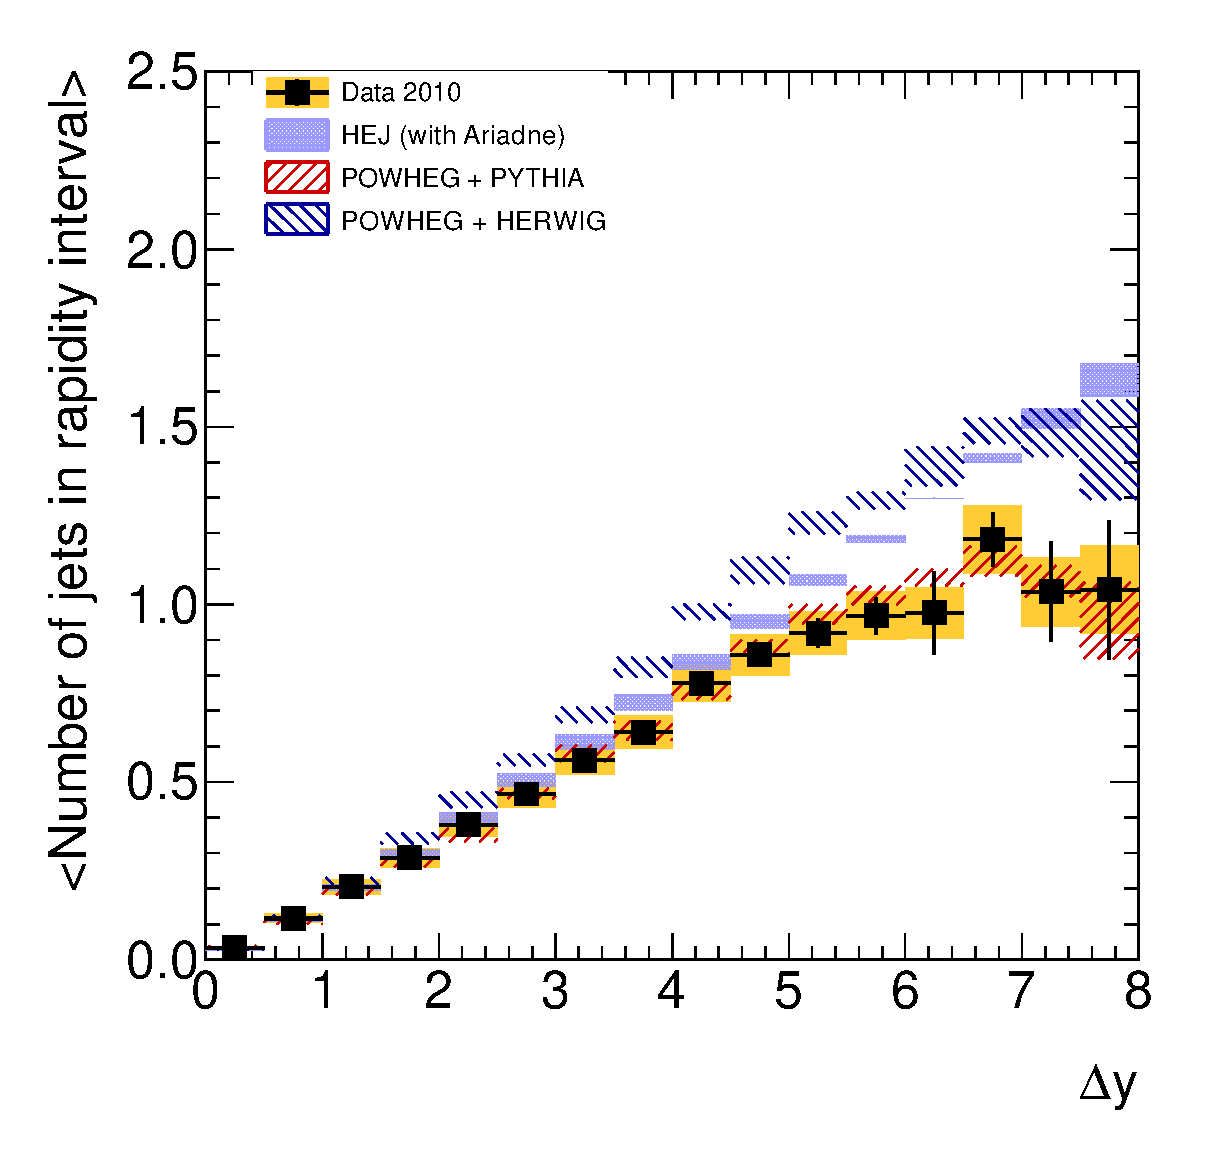
\includegraphics[width=\mediumfigwidth]{chapters/azimuthal-decorrelation/nGapJets_YDist.eps}
  \caption{Mean number of jets in the gap as a function of \DeltaY. The veto scale
           is set to \Qnought = \unit{20}{\GeV}. The unfolded data are compared
           to the \HEJ, \Powheg+\Pythia and \Powheg+\Herwig. The errors are as
           described in \FigureRef{fig:azimuthal-decorrelation:gap_fraction_theory}.}
  \label{fig:azimuthal-decorrelation:nGapJets_theory}
\end{figure}

\section{Summary}
The different \MC event generators show certain consistencies in their predictions
across each of these distributions. \Pythia tends to give the best description of
the data while \Herwigpp and \Alpgen both overestimate activity in the gap and hence
underestimate the gap fraction, particularly at high \DeltaY and low \Qnought. All
generators give a reasonable description of the
\meanCosDPhi and \meanCosTwoDPhi distributions, with the largest differences tending
to occur at the largest \DeltaY; the \meanCosTwoDPhi distributions also shows significant
shape differences between \Pythia and unfolded data. The \xs distributions show reasonable agreement between
data and leading order \MC generator predictions.

For the \xs distributions, reasonable agreement is seen between each of these
leading order \MC generators and the unfolded data, although statistics are limited
at large \DeltaY and low \DeltaPhi. This agreement comes despite the fact that no
correction has been made for soft effects.

These distributions will soon be augmented by the replacement of leading-order
\MC predictions by next-to-leading order predictions from \Powheg and \HEJ and
will then be considered for approval as an \ATLAS publication.
